\section{}

\textbf{Tiempo de lectura:} \{s14-reading-time\}

El \textbf{planificador de la CPU}{} o \textbf{planificador de corto
plazo}{} tiene la misión de seleccionar de la \textbf{cola de
preparados} el siguiente proceso o hilo de núcleo a ejecutar. En dicha
cola suelen estar los PCB ---o TCB--- de todos los procesos ---o hilos
de núcleo--- que esperan una oportunidad para usar la CPU. Aunque se
suele pensar en la \textbf{cola de preparados} como una cola FIFO, no
tiene por qué ser así, como veremos más adelante, ya que existen mejores
estrategias para seleccionar la próxima tarea a ejecutar.

En este capítulo hablaremos de procesos y de cómo son seleccionados por
el planificador de la CPU. Sin embargo, debemos tener en cuenta que en
los sistemas operativos multihilo con la librería de hilos implementada
en el núcleo ---categoría a la que pertenecen todos los sistemas
modernos--- la unidad de trabajo de la CPU es el hilo. Así que todo lo
que comentemos a partir de ahora sobre la planificación de procesos en
la CPU, realmente se aplica a los hilos y no a los procesos en los
sistemas operativos modernos.

En cualquier caso, sea cual sea el algoritmo de planificación utilizado,
este debe ser muy rápido, ya que es ejecutado con mucha frecuencia
---aproximadamente una vez cada 100 milisegundos---.

\section{Planificación
expropiativa}\label{_planificaciuxf3n_expropiativa}

{} El planificador deben ser invocado necesariamente en los siguientes
casos, dado que en ellos la CPU queda libre y es conveniente
aprovecharla planificando otro proceso, en lugar de dejarla desocupada:

\begin{enumerate}
\def\labelenumi{\arabic{enumi}.}
\item
  Cuando un proceso pasa de \textbf{ejecutando} a \textbf{esperando}.
  Por ejemplo, por solicitar una operación de E/S, esperar a que un hijo
  termine, esperar en un semáforo, etc.
\item
  Cuando un proceso termina.
\end{enumerate}

Cuando el planificador de la CPU es invocado solo en los casos
anteriores, decimos que tenemos un sistema operativo con
\textbf{planificación cooperativa}{} o \textbf{no expropiativa}{}.

En la \textbf{planificación cooperativa} cuando la CPU es asignada a un
proceso, este la acapara hasta terminar o hasta pasar al estado de
\textbf{esperando}.

La \textbf{planificación cooperativa} no requiere de ningún hardware
especial, por lo que en algunas plataformas puede ser la única opción.
Por ello estaba presente en los sistemas operativos más antiguos, como
\href{https://es.wikipedia.org/wiki/Windows_3.1x}{Windows 3.x} y
\href{https://es.wikipedia.org/wiki/Mac_OS}{Mac OS} ---que no debemos
confundir con el actual \{macos\}---.

Sin embargo, las decisiones de planificación también pueden ser tomadas
en otros dos casos:

\begin{enumerate}
\def\labelenumi{\arabic{enumi}.}
\item
  Cuando ocurre una interrupción del temporizador, lo que permite
  detectar si un proceso lleva demasiado tiempo ejecutándose.
\item
  Cuando un proceso pasa de \textbf{esperando} a \textbf{preparado}. Por
  ejemplo, porque para un proceso ha terminado la operación de E/S por
  la que estaba esperando.
\end{enumerate}

Cuando el planificador es invocado en los cuatro casos decimos que
tenemos \textbf{planificación expropiativa}{} o \textbf{apropiativa}{}.

La \textbf{planificación expropiativa} sí requiere de un soporte
adecuado por parte del hardware, por lo que se utiliza en los sistemas
operativos modernos. Ejemplos de estos sistemas son Microsoft Windows
---desde Windows 95--- Linux, macOS, y todos los UNIX modernos.

La utilización de un \textbf{planificador expropiativo} introduce
algunas dificultades adicionales:

\begin{itemize}
\item
  Puesto que un proceso puede ser expropiado en cualquier momento ---sin
  que pueda hacer nada para evitarlo--- el sistema operativo debe
  proporcionar \emph{mecanismos de sincronización} (véase el
  \hyperref[sincronizaciuxf3n]{???}) para coordinar el acceso a datos
  compartidos que podrían estar siendo modificados por el proceso que
  abandona la CPU y que puede necesitar el que entra en ella.
\item
  ¿Qué ocurre si un proceso va a ser expropiado en el preciso momento en
  el que se está ejecutando una llamada al sistema? No debemos olvidar
  que dentro del núcleo se manipulan datos importantes, compartidos por
  todo el sistema, que deben permanecer consistentes en todo momento.
\end{itemize}

Para resolver esta cuestión la solución más sencilla es impedir la
expropiación dentro del núcleo. Es decir, el cambio de contexto ---que
sacaría al proceso actual de la CPU y metería al siguiente--- no ocurre
inmediatamente, sino que se retrasa hasta que la llamada al sistema se
completa o se bloquea poniendo al proceso en el estado de
\emph{esperando}. Esto permite núcleos simples y garantiza que las
estructuras del mismo permanezcan consistentes, pero es una estrategia
muy pobre para sistemas de tiempo real o multiprocesador. Exploraremos
otras soluciones más adelante (véase el
\hyperref[_planificaciuxf3n_de_tiempo_real]{Planificación de tiempo
real}).

\section{El asignador}\label{_el_asignador}

El \textbf{{}asignador} es el componente que da el control de la CPU al
proceso seleccionado por el planificador de corto plazo. Esta tarea
implica realizar las siguientes funciones:

\begin{itemize}
\item
  Cambiar el contexto.
\item
  Cambiar al modo usuario.
\item
  Saltar al punto adecuado del programa para continuar la ejecución del
  proceso.
\end{itemize}

Puesto que el \textbf{asignador} es invocado para cada intercambio de
procesos en la CPU, es necesario que el tiempo que tarda en detener un
proceso e iniciar otro sea lo más corto posible. Al tiempo que
transcurre desde que un proceso es escogido para ser planificado en la
CPU hasta que es asignado a la misma se lo denomina \textbf{latencia de
asignación}{}.

\section{Criterios de
planificación}\label{_criterios_de_planificaciuxf3n}

Los diferentes algoritmos de planificación de la CPU tienen diversas
propiedades que pueden favorecer a una clase de procesos respecto a
otra. Por ello es interesante disponer de algún criterio para poder
comparar los algoritmos y determinar cuál es el mejor.

Se han sugerido muchos criterios para comparar los algoritmos de
planificación de CPU. La elección de uno u otro puede suponer una
diferencia sustancial a la hora de juzgar qué algoritmo es el mejor.

A continuación presentamos los criterios más comunes.

\subsection{Criterios a maximizar}\label{_criterios_a_maximizar}

Los algoritmos de planificación son mejores cuanto mayor es su valor
para los siguientes criterios.

\subsubsection{Uso de CPU}\label{_uso_de_cpu}

{} Un buen planificador debería mantener la CPU lo más ocupada posible.
El \textbf{uso de CPU} es la proporción de tiempo que se usa la CPU en
un periodo de tiempo determinado. Se suele indicar en tanto por ciento.

\["Uso de CPU" = 100 "Tiempo que la CPU permanece ocupada" / "Tiempo durante el que se toma la medida" "%"
\]

\subsubsection{Tasa de procesamiento}\label{_tasa_de_procesamiento}

{} Cuando la CPU está ocupada es porque el trabajo se está haciendo. Por
tanto, una buena medida del volumen de trabajo realizado puede ser el
número de tareas o procesos terminados por unidad de tiempo. A dicha
magnitud es a la que denominamos como \textbf{tasa de procesamiento}.

\["Tasa de procesamiento" = "Numero de procesos terminados" / "Tiempo durante el que se toma la medida" "procesos/s"\]

\subsection{Criterios a minimizar}\label{_criterios_a_minimizar}

Los algoritmos de planificación son mejores cuanto menor es su valor
para los siguientes criterios.

\begin{description}
\item[Tiempo de ejecución{}]
Es el intervalo de tiempo que transcurre desde que el proceso es cargado
hasta que termina.
\item[Tiempo de espera{}]
Es la suma de tiempos que el proceso permanece a la espera en la
\textbf{cola de preparados}. Esta medida de tiempo no incluye el tiempo
de espera debido a las operaciones de E/S.
\item[Tiempo de respuesta{}]
Es el intervalo de tiempo que transcurre desde que se lanza un evento
---se pulsa una tecla, se hace clic con el ratón o llega un paquete por
la interfaz de red--- hasta que se produce la primera respuesta del
proceso.
\end{description}

El \textbf{tiempo de respuesta} mide el tiempo que se tarda en responder
y no el tiempo de E/S. Mientras que el \textbf{tiempo de ejecución} sí
incluye el tiempo que consumen las operaciones de E/S, por lo que suele
estar limitado por la velocidad de los dispositivos E/S.

\subsection{Elección del criterio
adecuado}\label{_elecciuxf3n_del_criterio_adecuado}

En función del tipo de sistema o de la clase de trabajos que se van a
ejecutar puede ser conveniente medir la eficiencia del sistema usando un
criterio u otro. Esto a su vez beneficiará a unos algoritmos de
planificación frente a otros, indicándonos cuáles son los más eficientes
para nuestra clase de trabajos en particular.

En general podemos encontrar dos clases de trabajos para los que puede
ser necesario evaluar la eficiencia del sistema de manera diferente: los
trabajos interactivos y los que no lo son.

\subsubsection{Sistemas interactivos}\label{_sistemas_interactivos}

En los sistemas interactivos ---ya sean sistemas de escritorio o
\emph{mainframes} de tiempo compartido--- los procesos pasan la mayor
parte del tiempo esperando algún tipo de entrada por parte de los
usuarios.

En este tipo de sistemas, el \textbf{tiempo de ejecución} no suele ser
el mejor criterio para determinar la bondad de un algoritmo de
planificación, ya que viene determinado en gran medida por la velocidad
de la entrada de los usuarios. Por el contrario, se espera que el
sistema reaccione lo antes posible a las órdenes recibidas, lo que hace
que el \textbf{tiempo de respuesta} sea un criterio más adecuado para
evaluar al planificador de la CPU.

Generalmente, el \textbf{tiempo de respuesta} se reduce cuando el tiempo
que pasan los procesos interactivos en la \textbf{cola de preparados}
también lo hace ---tras haber sido puestos ahí por la ocurrencia de
algún evento--- por lo que también puede ser una buena idea utilizar
como criterio el \textbf{tiempo de espera}.

Esta selección de criterios no solo es adecuada para los sistemas
interactivos, ya que existen muchos otros casos donde es interesante
seleccionar un planificador de la CPU que minimice el tiempo de
respuesta. Esto, por ejemplo, ocurre con algunos servicios en red, como:
sistemas de mensajería instantánea, videoconferencia, servidores de
videojuegos, etc.

\subsubsection{Sistemas no
interactivos}\label{_sistemas_no_interactivos}

Por el contrario, en los antiguos \emph{mainframes} de procesamiento por
lotes y multiprogramados, en los superordenadores que realizan complejas
simulaciones físicas y en los grandes centros de datos de proveedores de
Internet como Google, lo de menos es el tiempo de respuesta y lo
realmente importante es completar cada tarea en el menor tiempo posible.
Por eso en ese tipo de sistemas es aconsejable utilizar criterios tales
como el \textbf{tiempo de ejecución} o la \textbf{tasa de
procesamiento}.

\subsubsection{Promedio o varianza del
criterio}\label{_promedio_o_varianza_del_criterio}

Obviamente estos criterios varían de un proceso a otro, por lo que
normalmente lo que se busca es optimizar los valores promedios en el
sistema.

Sin embargo, no debemos olvidar que en muchos casos puede ser más
conveniente optimizar el máximo y mínimo de dichos valores antes que el
promedio. Por ejemplo, en los sistemas interactivos es más importante
minimizar la \textbf{varianza en el tiempo de respuesta} que el
\textbf{tiempo de respuesta promedio}, puesto que para los usuarios un
sistema con un tiempo de respuesta predecible es más deseable que uno
muy rápido en promedio pero con una varianza muy alta.

\section{Ciclo de ráfagas de CPU y de
E/S}\label{_ciclo_de_ruxe1fagas_de_cpu_y_de_es}

El éxito de la planificación de CPU depende en gran medida de la
siguiente propiedad que podemos observar en hilos o procesos:

\emph{La ejecución de un hilo o proceso consiste en ciclos de CPU y
esperas de E/S, de forma que alternan entre estos dos estados.}

\emph{La ejecución empieza con una ráfaga de CPU, seguida por una ráfaga
de E/S, que a su vez es seguida por otra de CPU y así sucesivamente.}
\emph{Finalmente, la última ráfaga de CPU finaliza con una llamada al
sistema ---generalmente \{clang\_exit\}--- para terminar la ejecución
del proceso.}

\begin{figure}
\centering
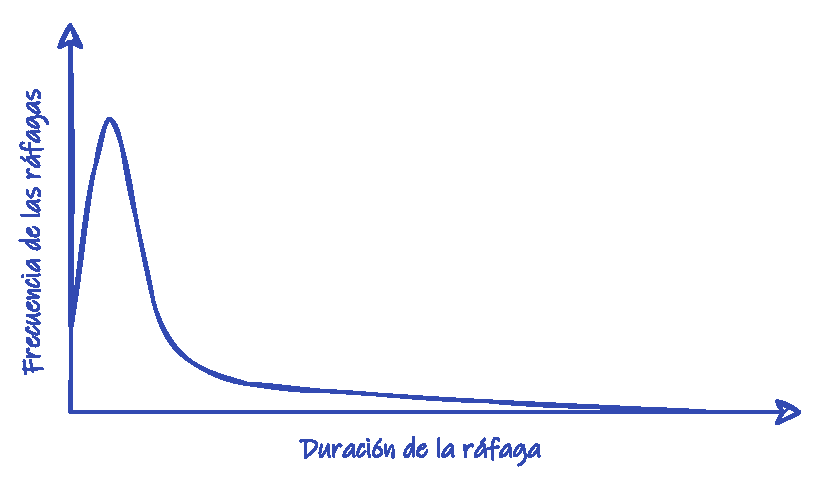
\includegraphics[width=0.8\textwidth]{media/C14_planificación/histogramas_tiempo_de_ráfagas.pdf}
\caption{Histograma de los tiempos de las ráfagas de
CPU.}\label{fig-ruxe1fagas-de-cpu}
\end{figure}

La curva que relaciona la frecuencia de las ráfagas de CPU con la
duración de las mismas tiende a ser exponencial o hiperexponencial
(véase la \hyperref[fig-ruxe1fagas-de-cpu]{Histograma de los tiempos de
las ráfagas de CPU.}) aunque varía enormemente entre tipos de tareas y
sistemas informáticos distintos. Esto significa que los procesos se
pueden clasificar entre aquellos que presentan un gran número de ráfagas
de CPU cortas o aquellos con un pequeño número de ráfagas de CPU largas.

Concretamente:

\begin{itemize}
\item
  Decimos que un proceso es \textbf{limitado por la E/S} cuando presenta
  muchas ráfagas de CPU cortas, debido a que si es así, es porque pasa
  la mayor parte del tiempo esperando por la E/S.
\item
  Decimos que un proceso está \textbf{limitado por la CPU} cuando
  presenta pocas ráfagas de CPU largas, debido a que si es así, es
  porque hace un uso intensivo de la misma y a penas pasa tiempo
  esperando por la E/S.
\end{itemize}

Esta distinción entre tipos de procesos puede ser importante en la
selección de un algoritmo de planificación de CPU adecuado, puesto que,
por lo general el algoritmo escogido debe planificar antes a los
procesos limitados por la E/S, evitando así que los procesos limitados
por la CPU ---que son los que tienden a usarla más tiempo--- la
acaparen.

Si esto último ocurriera, los procesos limitados por la E/S se
acumularían en la \textbf{cola de preparados}, dejando vacías las colas
de dispositivos. Este fenómeno, que provoca una infrautilización de los
dispositivos de E/S, se denomina \textbf{{}efecto convoy}.

Planificar primero a los procesos limitados por la E/S tiene además dos
efectos muy positivos:

\begin{itemize}
\item
  Los procesos interactivos son generalmente procesos limitados por la
  E/S, por lo que planificarlos primero hace que mejore el tiempo de
  respuesta.
\item
  Generalmente el tiempo de espera promedio se reduce cuando se
  planifican primero los procesos con ráfagas de CPU cortas. Según las
  definiciones anteriores, estos procesos son precisamente los limitados
  por la E/S.
\end{itemize}

\section{Algoritmos de planificación de la
CPU}\label{_algoritmos_de_planificaciuxf3n_de_la_cpu}

A continuación ilustraremos algunos de los algoritmos de planificación
de CPU más comunes. Lo haremos considerando que cada proceso tiene una
única ráfaga de CPU. Sin embargo, no debemos olvidar que para ser
precisos necesitaríamos utilizar muchos más procesos, donde cada uno
estuviera compuesto de una secuencia de miles de ráfagas alternativas de
CPU y de E/S.

\subsection{Planificación FCFS}\label{_planificaciuxf3n_fcfs}

{} En la planificación \textbf{{}FCFS} (\emph{First Come, First Served})
o \textbf{primero que llega, primero servido} la cola es FIFO:

\begin{itemize}
\item
  Los procesos que llegan se colocan al final de la cola que les
  corresponde.
\item
  El proceso asignado a la CPU se coge siempre del principio de la cola
  seleccionada.
\item
  Es un algoritmo \textbf{cooperativo}, puesto que un proceso mantiene
  la CPU hasta que decide liberarla voluntariamente ---recordemos que la
  ráfaga de CPU llega a su fin porque el proceso termina o solicita
  alguna operación que lo lleva el estado \textbf{esperando}---.
\end{itemize}

Ilustremos el algoritmo con un ejemplo. Supongamos que 4 procesos llegan
a la \textbf{cola de preparados} en los tiempos indicados en la
\hyperref[tabla-problema-fcfs]{Problema de planificación de la CPU
mediante algoritmo FCFS.}. Además, aunque es difícil tener un
conocimiento a priori del tiempo de la ráfaga de CPU de cada proceso,
vamos a suponer que también son conocidos.

\begin{longtable}[]{@{}
  >{\raggedright\arraybackslash}p{(\linewidth - 4\tabcolsep) * \real{0.3333}}
  >{\raggedright\arraybackslash}p{(\linewidth - 4\tabcolsep) * \real{0.3333}}
  >{\raggedright\arraybackslash}p{(\linewidth - 4\tabcolsep) * \real{0.3333}}@{}}
\caption{Problema de planificación de la CPU mediante algoritmo
FCFS.}\label{tabla-problema-fcfs}\tabularnewline
\toprule\noalign{}
\begin{minipage}[b]{\linewidth}\centering
Proceso
\end{minipage} & \begin{minipage}[b]{\linewidth}\centering
Tiempo de llegada (ms)
\end{minipage} & \begin{minipage}[b]{\linewidth}\centering
Tiempo de ráfaga de CPU (ms)
\end{minipage} \\
\midrule\noalign{}
\endfirsthead
\toprule\noalign{}
\begin{minipage}[b]{\linewidth}\centering
Proceso
\end{minipage} & \begin{minipage}[b]{\linewidth}\centering
Tiempo de llegada (ms)
\end{minipage} & \begin{minipage}[b]{\linewidth}\centering
Tiempo de ráfaga de CPU (ms)
\end{minipage} \\
\midrule\noalign{}
\endhead
\bottomrule\noalign{}
\endlastfoot
P1 & 0 & 24 \\
P2 & 1 & 3 \\
P3 & 2 & 3 \\
P4 & 3 & 2 \\
\end{longtable}

En la siguiente figura podemos ver el
\href{https://es.wikipedia.org/wiki/Diagrama_de_Gantt}{diagrama de
Gantt} de la planificación considerando que se utiliza el algoritmo
\textbf{FCFS}:

\begin{figure}
\centering
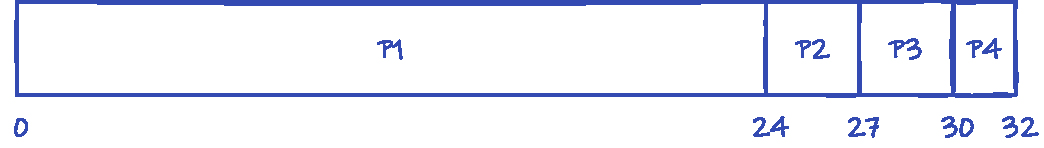
\includegraphics[width=0.8\textwidth]{media/C14_planificación/fcfs1.pdf}
\caption{}
\end{figure}

Utilizando el diagrama anterior, podemos calcular fácilmente los
\textbf{tiempos de espera y de ejecución promedio}:

\begin{longtable}[]{@{}
  >{\raggedright\arraybackslash}p{(\linewidth - 10\tabcolsep) * \real{0.2857}}
  >{\raggedright\arraybackslash}p{(\linewidth - 10\tabcolsep) * \real{0.1429}}
  >{\raggedright\arraybackslash}p{(\linewidth - 10\tabcolsep) * \real{0.1429}}
  >{\raggedright\arraybackslash}p{(\linewidth - 10\tabcolsep) * \real{0.1429}}
  >{\raggedright\arraybackslash}p{(\linewidth - 10\tabcolsep) * \real{0.1429}}
  >{\raggedright\arraybackslash}p{(\linewidth - 10\tabcolsep) * \real{0.1429}}@{}}
\toprule\noalign{}
\begin{minipage}[b]{\linewidth}\centering
Proceso
\end{minipage} & \begin{minipage}[b]{\linewidth}\centering
Instante de finalización (ms)
\end{minipage} &
\multicolumn{2}{>{\centering\arraybackslash}p{(\linewidth - 10\tabcolsep) * \real{0.2857} + 2\tabcolsep}}{\begin{minipage}[b]{\linewidth}\centering
Tiempo de espera (ms)
\end{minipage} &
\multicolumn{2}{>{\centering\arraybackslash}p{(\linewidth - 10\tabcolsep) * \real{0.2857} + 2\tabcolsep}@{}}{\begin{minipage}[b]{\linewidth}\centering
Tiempo de ejecución (ms)
\end{minipage} \\
\midrule\noalign{}
\endhead
\bottomrule\noalign{}
\endlastfoot
P1 & 24 & {(0-0)=} & 0 & {(24-0)=} & 24 \\
P2 & 27 & {(24-1)=} & 23 & {(27-1)=} & 26 \\
P3 & 30 & {(27-2)=} & 25 & {(30-2)=} & 28 \\
P4 & 32 & {(30-3)=} & 27 & {(32-3)=} & 29 \\
\end{longtable}

Lo interesante es que el resultado cambia si los procesos llegan en otro
orden. Por ejemplo, P1 podría llegar el último:

\begin{longtable}[]{@{}
  >{\raggedright\arraybackslash}p{(\linewidth - 4\tabcolsep) * \real{0.3333}}
  >{\raggedright\arraybackslash}p{(\linewidth - 4\tabcolsep) * \real{0.3333}}
  >{\raggedright\arraybackslash}p{(\linewidth - 4\tabcolsep) * \real{0.3333}}@{}}
\toprule\noalign{}
\begin{minipage}[b]{\linewidth}\centering
Proceso
\end{minipage} & \begin{minipage}[b]{\linewidth}\centering
Tiempo de llegada (ms)
\end{minipage} & \begin{minipage}[b]{\linewidth}\centering
Tiempo de ráfaga de CPU (ms)
\end{minipage} \\
\midrule\noalign{}
\endhead
\bottomrule\noalign{}
\endlastfoot
P2 & 0 & 3 \\
P3 & 1 & 3 \\
P4 & 2 & 2 \\
P1 & 3 & 24 \\
\end{longtable}

Entonces el resultado de la planificación sería el que se muestra en la
siguiente figura:

\begin{figure}
\centering
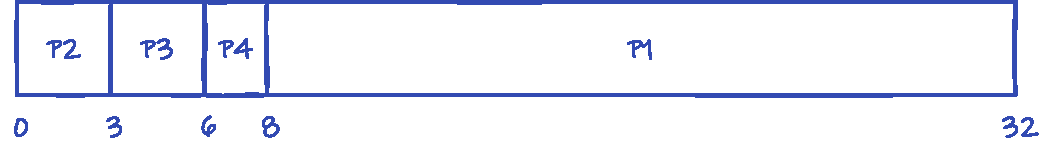
\includegraphics[width=0.8\textwidth]{media/C14_planificación/fcfs2.pdf}
\caption{}
\end{figure}

Y los \textbf{tiempos de espera y ejecución promedio} correspondientes
serían:

\begin{longtable}[]{@{}
  >{\raggedright\arraybackslash}p{(\linewidth - 10\tabcolsep) * \real{0.2857}}
  >{\raggedright\arraybackslash}p{(\linewidth - 10\tabcolsep) * \real{0.1429}}
  >{\raggedright\arraybackslash}p{(\linewidth - 10\tabcolsep) * \real{0.1429}}
  >{\raggedright\arraybackslash}p{(\linewidth - 10\tabcolsep) * \real{0.1429}}
  >{\raggedright\arraybackslash}p{(\linewidth - 10\tabcolsep) * \real{0.1429}}
  >{\raggedright\arraybackslash}p{(\linewidth - 10\tabcolsep) * \real{0.1429}}@{}}
\toprule\noalign{}
\begin{minipage}[b]{\linewidth}\centering
Proceso
\end{minipage} & \begin{minipage}[b]{\linewidth}\centering
Instante de finalización (ms)
\end{minipage} &
\multicolumn{2}{>{\centering\arraybackslash}p{(\linewidth - 10\tabcolsep) * \real{0.2857} + 2\tabcolsep}}{\begin{minipage}[b]{\linewidth}\centering
Tiempo de espera (ms)
\end{minipage} &
\multicolumn{2}{>{\centering\arraybackslash}p{(\linewidth - 10\tabcolsep) * \real{0.2857} + 2\tabcolsep}@{}}{\begin{minipage}[b]{\linewidth}\centering
Tiempo de ejecución (ms)
\end{minipage} \\
\midrule\noalign{}
\endhead
\bottomrule\noalign{}
\endlastfoot
P2 & 3 & {(0-0)=} & 0 & {(3-0)=} & 3 \\
P3 & 6 & {(3-1)=} & 2 & {(6-1)=} & 5 \\
P4 & 8 & {(6-2)=} & 4 & {(8-2)=} & 6 \\
P1 & 32 & {(8-3)=} & 5 & {(32-3)=} & 29 \\
\end{longtable}

Aunque el tiempo total necesario para ejecutar las ráfagas de los 4
procesos, los criterios utilizados reflejan que el algoritmo se comporta
mucho mejor en el segundo caso. Por tanto, el algoritmo \textbf{FCFS} no
garantiza ni \textbf{tiempos de espera} ni de \textbf{ejecución}
mínimos, ya que pueden cambiar variar considerablemente con el orden en
el que llegan los procesos.

Además, el algoritmo \textbf{FCFS} sufre el llamado \textbf{{}efecto
convoy}. Para entenderlo, analicemos lo que está pasando en el ejemplo
de la \hyperref[tabla-problema-fcfs]{Problema de planificación de la CPU
mediante algoritmo FCFS.}:

\begin{enumerate}
\def\labelenumi{\arabic{enumi}.}
\item
  Al proceso P1 se le asigna la CPU. Durante el tiempo que P1 utiliza la
  CPU todos los otros procesos terminan sus operaciones de E/S y pasan a
  la \textbf{cola de preparados}. Por tanto, mientras los procesos
  esperan para utilizar la CPU, los dispositivos de E/S permanecen
  desocupados.
\item
  El proceso P1 termina de usar la CPU y pasa a una cola de
  dispositivos.
\item
  El resto de procesos P, que tienen ráfagas de CPU cortas, se ejecutan
  rápidamente y pasan a las colas de dispositivos. Por tanto, la CPU
  permanecerá vacía hasta que algún proceso termine la operación de E/S
  solicitada.
\item
  El proceso P1 pasa a la \textbf{cola de preparados} y se le asigna la
  CPU. Con el tiempo el resto de procesos terminarán sus operaciones y,
  nuevamente, tienen que esperar en la \textbf{cola de preparados} a que
  el proceso P1 termine de utilizarla.
\end{enumerate}

Esto nos permite llegar a la conclusión de que en cierto orden de
llegada la mayor parte de los procesos esperan constantemente detrás de
uno para poder realizar su trabajo. Esto reduce la utilización de la CPU
y de los dispositivos de E/S por debajo de lo que sería posible, si los
procesos más cortos se ejecutasen primero.

\subsection{Planificación SJF}\label{_planificaciuxf3n_sjf}

{} La planificación \textbf{{}SJF} (\emph{Shortest-Job First}) o
\textbf{primero el más corto}, consiste en:

\begin{enumerate}
\def\labelenumi{\arabic{enumi}.}
\item
  Se asocia con cada proceso la longitud de tiempo de su siguiente
  ráfaga de CPU.
\item
  Cuando la CPU está disponible, se pone \textbf{ejecutando} el proceso
  de menor ráfaga de CPU.
\item
  Si dos procesos tienen ráfagas de una misma longitud, se utiliza el
  algoritmo \textbf{FCFS} ---entre ellos, el que lleva más tiempo en la
  \textbf{cola de preparados}---.
\item
  Es un algoritmo \textbf{cooperativo}, puesto que un proceso mantiene
  la CPU hasta que decide liberarla voluntariamente.
\end{enumerate}

Ilustremos el algoritmo con un ejemplo:

\begin{longtable}[]{@{}
  >{\raggedright\arraybackslash}p{(\linewidth - 4\tabcolsep) * \real{0.3333}}
  >{\raggedright\arraybackslash}p{(\linewidth - 4\tabcolsep) * \real{0.3333}}
  >{\raggedright\arraybackslash}p{(\linewidth - 4\tabcolsep) * \real{0.3333}}@{}}
\toprule\noalign{}
\begin{minipage}[b]{\linewidth}\centering
Proceso
\end{minipage} & \begin{minipage}[b]{\linewidth}\centering
Tiempo de llegada (ms)
\end{minipage} & \begin{minipage}[b]{\linewidth}\centering
Tiempo de ráfaga de CPU (ms)
\end{minipage} \\
\midrule\noalign{}
\endhead
\bottomrule\noalign{}
\endlastfoot
P1 & 0 & 6 \\
P2 & 1 & 8 \\
P3 & 2 & 7 \\
P4 & 3 & 3 \\
\end{longtable}

Considerando que se utiliza el algoritmo \textbf{SJF} obtendremos el
siguiente diagrama de Gantt:

\begin{figure}
\centering
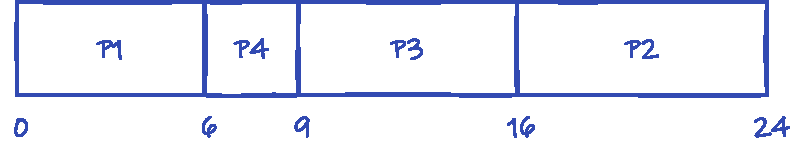
\includegraphics[width=0.8\textwidth]{media/C14_planificación/sjf.pdf}
\caption{}
\end{figure}

Con los \textbf{tiempos de espera y ejecución promedio}
correspondientes:

\begin{longtable}[]{@{}
  >{\raggedright\arraybackslash}p{(\linewidth - 10\tabcolsep) * \real{0.2857}}
  >{\raggedright\arraybackslash}p{(\linewidth - 10\tabcolsep) * \real{0.1429}}
  >{\raggedright\arraybackslash}p{(\linewidth - 10\tabcolsep) * \real{0.1429}}
  >{\raggedright\arraybackslash}p{(\linewidth - 10\tabcolsep) * \real{0.1429}}
  >{\raggedright\arraybackslash}p{(\linewidth - 10\tabcolsep) * \real{0.1429}}
  >{\raggedright\arraybackslash}p{(\linewidth - 10\tabcolsep) * \real{0.1429}}@{}}
\toprule\noalign{}
\begin{minipage}[b]{\linewidth}\centering
Proceso
\end{minipage} & \begin{minipage}[b]{\linewidth}\centering
Instante de finalización (ms)
\end{minipage} &
\multicolumn{2}{>{\centering\arraybackslash}p{(\linewidth - 10\tabcolsep) * \real{0.2857} + 2\tabcolsep}}{\begin{minipage}[b]{\linewidth}\centering
Tiempo de espera (ms)
\end{minipage} &
\multicolumn{2}{>{\centering\arraybackslash}p{(\linewidth - 10\tabcolsep) * \real{0.2857} + 2\tabcolsep}@{}}{\begin{minipage}[b]{\linewidth}\centering
Tiempo de ejecución (ms)
\end{minipage} \\
\midrule\noalign{}
\endhead
\bottomrule\noalign{}
\endlastfoot
P1 & 6 & {(0-0)=} & 0 & {(6-0)=} & 6 \\
P2 & 24 & {(16-1)=} & 15 & {(24-1)=} & 23 \\
P3 & 16 & {(9-2)=} & 7 & {(16-2)=} & 14 \\
P4 & 9 & {(6-3)=} & 3 & {(9-3)=} & 6 \\
\end{longtable}

Sin embargo, si hubiéramos utilizado el algoritmo \textbf{FCFS}:

\begin{figure}
\centering
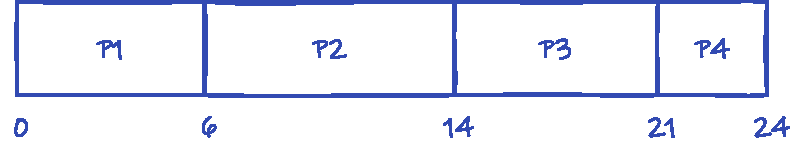
\includegraphics[width=0.8\textwidth]{media/C14_planificación/fcfs-sjf.pdf}
\caption{}
\end{figure}

\begin{longtable}[]{@{}
  >{\raggedright\arraybackslash}p{(\linewidth - 10\tabcolsep) * \real{0.2857}}
  >{\raggedright\arraybackslash}p{(\linewidth - 10\tabcolsep) * \real{0.1429}}
  >{\raggedright\arraybackslash}p{(\linewidth - 10\tabcolsep) * \real{0.1429}}
  >{\raggedright\arraybackslash}p{(\linewidth - 10\tabcolsep) * \real{0.1429}}
  >{\raggedright\arraybackslash}p{(\linewidth - 10\tabcolsep) * \real{0.1429}}
  >{\raggedright\arraybackslash}p{(\linewidth - 10\tabcolsep) * \real{0.1429}}@{}}
\toprule\noalign{}
\begin{minipage}[b]{\linewidth}\centering
Proceso
\end{minipage} & \begin{minipage}[b]{\linewidth}\centering
Instante de finalización (ms)
\end{minipage} &
\multicolumn{2}{>{\centering\arraybackslash}p{(\linewidth - 10\tabcolsep) * \real{0.2857} + 2\tabcolsep}}{\begin{minipage}[b]{\linewidth}\centering
Tiempo de espera (ms)
\end{minipage} &
\multicolumn{2}{>{\centering\arraybackslash}p{(\linewidth - 10\tabcolsep) * \real{0.2857} + 2\tabcolsep}@{}}{\begin{minipage}[b]{\linewidth}\centering
Tiempo de ejecución (ms)
\end{minipage} \\
\midrule\noalign{}
\endhead
\bottomrule\noalign{}
\endlastfoot
P1 & 6 & {(0-0)=} & 0 & {(6-0)=} & 6 \\
P2 & 14 & {(6-1)=} & 5 & {(14-1)=} & 13 \\
P3 & 21 & {(14-2)=} & 12 & {(21-2)=} & 19 \\
P4 & 24 & {(21-3)=} & 18 & {(24-3)=} & 21 \\
\end{longtable}

El algoritmo \textbf{SJF} es óptimo en el sentido de que el
\textbf{tiempo de espera promedio} es mínimo, porque reduce más el
tiempo de espera de los procesos cortos y aumenta el de los procesos
largos. Además, así se evita el \textbf{efecto convoy}.

Sin embargo, la pregunta que debemos hacernos es cómo podemos conocer de
antemano la longitud de las ráfagas de CPU de un proceso, para usar esa
información durante la planificación. Sin analizar el código, el sistema
operativo no puede conocer el tiempo de una ráfaga hasta que esta no
termina de ejecutarse.

Por eso el algoritmo SJF se utiliza frecuentemente como planificador de
la \textbf{cola de trabajos}, donde se puede obligar al usuario a
especificar un tiempo de ejecución máximo, al enviar el trabajo a dicha
cola. En este caso, los usuarios tenderán a ajustar la estimación de
tiempo de ejecución, puesto que los que tengan tiempos más cortos serán
priorizados para ser ejecutados antes, frente a los de tiempos más
largos.

Para evitar que los usuarios hagan trampas indicando un tiempo de
ejecución más corto que el real, con el fin de que se planifique antes
su trabajo, se puede utilizar un temporizador para abortar los trabajos
que excedan el tiempo de ejecución indicado por el usuario. El error
puede ser notificado al usuario para que vuelva a enviar el trabajo con
una estimación más realista.

Para utilizar el algoritmo \textbf{SJF} en el planificador de la CPU, lo
único que se puede hacer es intentar predecir el tiempo de la siguiente
ráfaga de CPU. Por ejemplo, se puede utilizar un promedio ponderado
exponencial de los tiempos de las de ráfagas de CPU pasadas:

\[tau_(n+1) = alpha*t_n + (1 - alpha)*tau_n, 0 le alpha le 1\]

donde:

\begin{itemize}
\item
  \(tau_(n+1)\) es la estimación de tiempo de la siguiente ráfaga de CPU
\item
  \(t_n\) es el tiempo real de la última ráfaga
\item
  \(alpha\) es el peso relativo del tiempo real de la última ráfaga.
\item
  \(tau_(n)\) es la estimación de tiempo de la última ráfaga.
\end{itemize}

La expresión es recursiva, dado que \(tau_n\) se calcula usando la
ecuación con \(t_(n-1)\) y \(tau_(n-1)\); que a su vez depende de
\(t_(n-2)\) y \(tau_(n-2)\), y así sucesivamente.

Si desarrollamos la fórmula sustituyendo los valores, veremos que
\(t_n\) se pondera con \(alpha\), \(t_(n-1)\) con \((1 - alpha)alpha\),
\(t_(n-2)\) con \((1 - alpha)^2alpha\), y así sucesivamente:

\[tau_(n+1) = alpha*t_n + (1 - alpha)*alpha*t_(n-1) + (1 - alpha)^2*alpha*t_(n-2) + ...\]

Si \(alpha\) = 1, \(tau_(n+1)\) = \(alpha*t_n\), ignorando el resto del
histórico. En otro caso, dado que tanto \(alpha\) como \(1 - alpha\) son
menores de 1, cada término sucesivo tiene menor peso que su predecesor,
haciendo que los \(t_n\) contribuyan menos cuanto más alejados del
tiempo actual.

El problema es que todos estos cálculos consumen tiempo de CPU, cuando
el planificador debe ser lo más rápido posible, dado que se ejecuta con
mucha frecuencia.

\subsection{Planificación SRTF}\label{_planificaciuxf3n_srtf}

{} El algoritmo \textbf{SJF} es \textbf{cooperativo}, pero se puede
implementar de forma \textbf{expropiativa}, en cuyo caso se llama
\textbf{{}SRTF} (Shortest-Remaing-Time First). La diferencia está en lo
que ocurre cuando un nuevo proceso llega a la \textbf{cola de
preparados}.

En \textbf{SRTF} se compara el tiempo de la siguiente ráfaga de CPU del
nuevo proceso, con el tiempo de ráfaga que le queda al proceso en
ejecución. Si la primera magnitud es inferior, el proceso que tiene la
CPU es expropiado y sustituido por el nuevo proceso. Mientras que en
\textbf{SJF} no se hace nada. Se espera que el proceso que actualmente
se está ejecutando termine su ráfaga de CPU voluntariamente.

Ilustremos el algoritmo con un ejemplo:

\begin{longtable}[]{@{}
  >{\raggedright\arraybackslash}p{(\linewidth - 4\tabcolsep) * \real{0.3333}}
  >{\raggedright\arraybackslash}p{(\linewidth - 4\tabcolsep) * \real{0.3333}}
  >{\raggedright\arraybackslash}p{(\linewidth - 4\tabcolsep) * \real{0.3333}}@{}}
\toprule\noalign{}
\begin{minipage}[b]{\linewidth}\centering
Proceso
\end{minipage} & \begin{minipage}[b]{\linewidth}\centering
Tiempo de llegada (ms)
\end{minipage} & \begin{minipage}[b]{\linewidth}\centering
Tiempo de ráfaga de CPU (ms)
\end{minipage} \\
\midrule\noalign{}
\endhead
\bottomrule\noalign{}
\endlastfoot
P1 & 0 & 8 \\
P2 & 1 & 4 \\
P3 & 2 & 9 \\
P4 & 3 & 5 \\
\end{longtable}

El resultado es el que se muestra en el siguiente diagrama de Gantt:

\begin{figure}
\centering
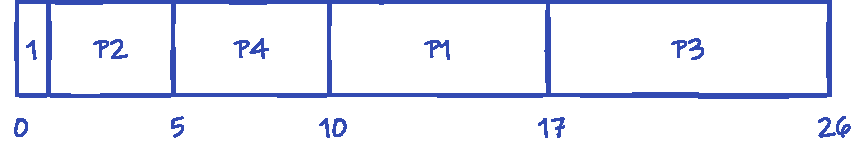
\includegraphics[width=0.8\textwidth]{media/C14_planificación/srtf.pdf}
\caption{}
\end{figure}

Y los tiempos de espera y ejecución promedio correspondientes serían:

\begin{longtable}[]{@{}
  >{\raggedright\arraybackslash}p{(\linewidth - 10\tabcolsep) * \real{0.2857}}
  >{\raggedright\arraybackslash}p{(\linewidth - 10\tabcolsep) * \real{0.1429}}
  >{\raggedright\arraybackslash}p{(\linewidth - 10\tabcolsep) * \real{0.1429}}
  >{\raggedright\arraybackslash}p{(\linewidth - 10\tabcolsep) * \real{0.1429}}
  >{\raggedright\arraybackslash}p{(\linewidth - 10\tabcolsep) * \real{0.1429}}
  >{\raggedright\arraybackslash}p{(\linewidth - 10\tabcolsep) * \real{0.1429}}@{}}
\toprule\noalign{}
\begin{minipage}[b]{\linewidth}\centering
Proceso
\end{minipage} & \begin{minipage}[b]{\linewidth}\centering
Instante de finalización (ms)
\end{minipage} &
\multicolumn{2}{>{\centering\arraybackslash}p{(\linewidth - 10\tabcolsep) * \real{0.2857} + 2\tabcolsep}}{\begin{minipage}[b]{\linewidth}\centering
Tiempo de espera (ms)
\end{minipage} &
\multicolumn{2}{>{\centering\arraybackslash}p{(\linewidth - 10\tabcolsep) * \real{0.2857} + 2\tabcolsep}@{}}{\begin{minipage}[b]{\linewidth}\centering
Tiempo de ejecución (ms)
\end{minipage} \\
\midrule\noalign{}
\endhead
\bottomrule\noalign{}
\endlastfoot
P1 & 17 & {(0-0) + (10-1)=} & 9 & {(17-0)=} & 17 \\
P2 & 5 & {(1-1)=} & 0 & {(5-1)=} & 4 \\
P3 & 26 & {(17-2)=} & 15 & {(26-2)=} & 24 \\
P4 & 10 & {(5-3)=} & 2 & {(10-3)=} & 7 \\
\end{longtable}

Es muy complicado predecir cuál de los dos algoritmos será mejor para un
conjunto concreto de procesos. Sin embargo, debemos tener en cuenta que
---aunque no lo estemos considerando en estos problemas--- un algoritmo
expropitativo, por lo general, provocará más cambios de contexto en los
que se perderá tiempo de CPU.

Los algoritmos expropiativos también suelen ofrecer mejores tiempos de
respuesta, puesto que un proceso que llega a la \textbf{cola de
preparados} puede ser asignado a la CPU sin esperar a que el proceso que
se ejecuta en ella actualmente termine su ráfaga de CPU.

\subsection{Planificación con
prioridades}\label{_planificaciuxf3n_con_prioridades}

{} En la \textbf{planificación con prioridades} se asocia una prioridad
a cada proceso, de tal forma que el de prioridad más alta es asignado a
la CPU. En caso de igual prioridad, se utiliza \textbf{FCFS}.

Las prioridades se suelen indicar con números enteros en un rango fijo.
Por ejemplo {[}0-7{]}, {[}0-31{]}, {[}0-139{]} o {[}0-4095{]}. En
algunos sistemas operativos los números más grandes representan mayor
prioridad, mientras que en otros son los procesos con números más
pequeños los que se planifican primero. En este curso utilizaremos la
convención de que a menor valor, mayor prioridad.

Si las prioridades se asignan en relación con el tiempo de la próxima
ráfaga de CPU, su comportamiento es el mismo que el del \textbf{SJF};
por lo que se considera a este último un caso particular de algoritmo de
\textbf{planificación con prioridades}.

El algoritmo de planificación con prioridades puede ser
\textbf{expropiativo} o \textbf{cooperativo}:

\begin{itemize}
\item
  En el caso \textbf{expropiativo}, cuando un proceso llega a la
  \textbf{cola de preparados} su prioridad es comparada con la del
  proceso en ejecución. Se expropia la CPU si la prioridad del nuevo
  proceso es superior a la prioridad del proceso que se ejecuta.
\item
  En el caso \textbf{cooperativo}, no se toma ninguna decisión cuando
  llega un proceso a la \textbf{cola de preparados}, solo cuando el que
  tiene asignada la CPU la abandona.
\end{itemize}

Supongamos que 5 procesos llegan a la cola de preparados en los tiempos
indicados en la \hyperref[tabla-problema-prioridad]{Problema de
planificación de la CPU mediante algoritmo de planificación con
prioridades.}. Como en los ejemplos anteriores, aunque es difícil tener
un conocimiento a priori del tiempo de las ráfagas de CPU, vamos a
suponer que son conocidos. Y también que a cada proceso se le asigna, de
alguna forma, una prioridad cuando llega a la \textbf{cola de
preparados}.

\begin{longtable}[]{@{}
  >{\raggedright\arraybackslash}p{(\linewidth - 6\tabcolsep) * \real{0.2500}}
  >{\raggedright\arraybackslash}p{(\linewidth - 6\tabcolsep) * \real{0.2500}}
  >{\raggedright\arraybackslash}p{(\linewidth - 6\tabcolsep) * \real{0.2500}}
  >{\raggedright\arraybackslash}p{(\linewidth - 6\tabcolsep) * \real{0.2500}}@{}}
\caption{Problema de planificación de la CPU mediante algoritmo de
planificación con
prioridades.}\label{tabla-problema-prioridad}\tabularnewline
\toprule\noalign{}
\begin{minipage}[b]{\linewidth}\centering
Proceso
\end{minipage} & \begin{minipage}[b]{\linewidth}\centering
Tiempo de llegada (ms)
\end{minipage} & \begin{minipage}[b]{\linewidth}\centering
Tiempo de ráfaga de CPU (ms)
\end{minipage} & \begin{minipage}[b]{\linewidth}\centering
Prioridad
\end{minipage} \\
\midrule\noalign{}
\endfirsthead
\toprule\noalign{}
\begin{minipage}[b]{\linewidth}\centering
Proceso
\end{minipage} & \begin{minipage}[b]{\linewidth}\centering
Tiempo de llegada (ms)
\end{minipage} & \begin{minipage}[b]{\linewidth}\centering
Tiempo de ráfaga de CPU (ms)
\end{minipage} & \begin{minipage}[b]{\linewidth}\centering
Prioridad
\end{minipage} \\
\midrule\noalign{}
\endhead
\bottomrule\noalign{}
\endlastfoot
P1 & 0 & 10 & 3 \\
P2 & 1 & 2 & 1 \\
P3 & 2 & 3 & 4 \\
P4 & 3 & 2 & 5 \\
P5 & 4 & 5 & 2 \\
\end{longtable}

En las condiciones anteriores, si utilizamos el algoritmo de
planificación por prioridades expropiativo, obtendremos el diagrama de
Gantt de la siguiente figura:

\begin{figure}
\centering
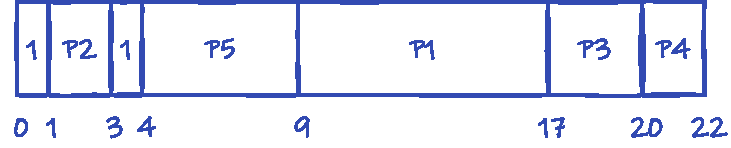
\includegraphics[width=0.8\textwidth]{media/C14_planificación/prioridad.pdf}
\caption{}
\end{figure}

Con los \textbf{tiempos de espera y ejecución promedio}
correspondientes:

\begin{longtable}[]{@{}
  >{\raggedright\arraybackslash}p{(\linewidth - 10\tabcolsep) * \real{0.2857}}
  >{\raggedright\arraybackslash}p{(\linewidth - 10\tabcolsep) * \real{0.1429}}
  >{\raggedright\arraybackslash}p{(\linewidth - 10\tabcolsep) * \real{0.1429}}
  >{\raggedright\arraybackslash}p{(\linewidth - 10\tabcolsep) * \real{0.1429}}
  >{\raggedright\arraybackslash}p{(\linewidth - 10\tabcolsep) * \real{0.1429}}
  >{\raggedright\arraybackslash}p{(\linewidth - 10\tabcolsep) * \real{0.1429}}@{}}
\toprule\noalign{}
\begin{minipage}[b]{\linewidth}\centering
Proceso
\end{minipage} & \begin{minipage}[b]{\linewidth}\centering
Instante de finalización (ms)
\end{minipage} &
\multicolumn{2}{>{\centering\arraybackslash}p{(\linewidth - 10\tabcolsep) * \real{0.2857} + 2\tabcolsep}}{\begin{minipage}[b]{\linewidth}\centering
Tiempo de espera (ms)
\end{minipage} &
\multicolumn{2}{>{\centering\arraybackslash}p{(\linewidth - 10\tabcolsep) * \real{0.2857} + 2\tabcolsep}@{}}{\begin{minipage}[b]{\linewidth}\centering
Tiempo de ejecución (ms)
\end{minipage} \\
\midrule\noalign{}
\endhead
\bottomrule\noalign{}
\endlastfoot
P1 & 4 & {(0-0) + (3-1) + (9-4)=} & 7 & {(17-0)=} & 17 \\
P2 & 3 & {(1-1)=} & 0 & {(3-1)=} & 2 \\
P3 & 20 & {(17-2)=} & 15 & {(20-2)=} & 18 \\
P4 & 22 & {(20-3)=} & 17 & {(22-3)=} & 19 \\
P5 & 9 & {(4-4)=} & 0 & {(9-4)=} & 5 \\
\end{longtable}

Mientras que si utilizamos el algoritmo de planificación por prioridades
cooperativo, obtendremos el diagrama de Gantt de la siguiente figura:

\begin{figure}
\centering
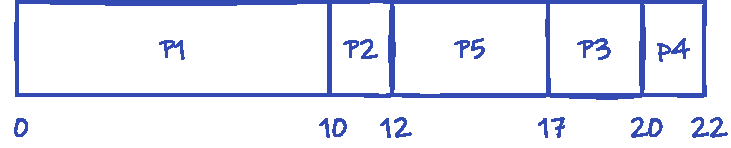
\includegraphics[width=0.8\textwidth]{media/C14_planificación/prioridad_cooperativo.pdf}
\caption{}
\end{figure}

Con los \textbf{tiempos de espera y ejecución promedio}
correspondientes:

\begin{longtable}[]{@{}
  >{\raggedright\arraybackslash}p{(\linewidth - 10\tabcolsep) * \real{0.2857}}
  >{\raggedright\arraybackslash}p{(\linewidth - 10\tabcolsep) * \real{0.1429}}
  >{\raggedright\arraybackslash}p{(\linewidth - 10\tabcolsep) * \real{0.1429}}
  >{\raggedright\arraybackslash}p{(\linewidth - 10\tabcolsep) * \real{0.1429}}
  >{\raggedright\arraybackslash}p{(\linewidth - 10\tabcolsep) * \real{0.1429}}
  >{\raggedright\arraybackslash}p{(\linewidth - 10\tabcolsep) * \real{0.1429}}@{}}
\toprule\noalign{}
\begin{minipage}[b]{\linewidth}\centering
Proceso
\end{minipage} & \begin{minipage}[b]{\linewidth}\centering
Instante de finalización (ms)
\end{minipage} &
\multicolumn{2}{>{\centering\arraybackslash}p{(\linewidth - 10\tabcolsep) * \real{0.2857} + 2\tabcolsep}}{\begin{minipage}[b]{\linewidth}\centering
Tiempo de espera (ms)
\end{minipage} &
\multicolumn{2}{>{\centering\arraybackslash}p{(\linewidth - 10\tabcolsep) * \real{0.2857} + 2\tabcolsep}@{}}{\begin{minipage}[b]{\linewidth}\centering
Tiempo de ejecución (ms)
\end{minipage} \\
\midrule\noalign{}
\endhead
\bottomrule\noalign{}
\endlastfoot
P1 & 10 & {(0-0)=} & 0 & {(10-0)=} & 10 \\
P2 & 12 & {(10-1)=} & 9 & {(12-1)=} & 11 \\
P3 & 20 & {(17-2)=} & 15 & {(20-2)=} & 18 \\
P4 & 22 & {(20-3)=} & 17 & {(22-3)=} & 19 \\
P5 & 17 & {(12-4)=} & 8 & {(17-4)=} & 13 \\
\end{longtable}

Que estos algoritmos ofrezcan mejores o peores resultados que otros,
obviamente depende de los criterios utilizados para asignar las
prioridades.

\subsubsection{Prioridades definidas internamente o
externamente}\label{_prioridades_definidas_internamente_o_externamente}

Hay dos maneras de asignar las prioridades:

\begin{itemize}
\item
  \textbf{Internamente}. Se utiliza una cualidad medible del proceso
  para calcular su prioridad. Por ejemplo, límites de tiempo,
  necesidades de memoria, número de archivos abiertos, tiempo estimado
  de ráfaga de CPU ---como en \textbf{SJF}--- o la proporción entre esta
  y el tiempo estimado de ráfaga de E/S.
\item
  \textbf{Externamente}. Las prioridades son fijadas por criterios
  externos al sistema operativo. Por ejemplo, la importancia del proceso
  para los usuarios, la cantidad de dinero pagada para el uso del
  sistema u otros factores políticos.
\end{itemize}

Algunas de estas formas de asignar las prioridades pueden ser fijas,
mientras que otras pueden ser variables. Es decir, un criterio externo
como es la importancia del proceso para los usuarios, puede dar lugar a
una prioridad que se asigna al crear el proceso y que no cambia durante
toda su ejecución. Por el contrario, un criterio como el tiempo de
ráfaga de CPU puede dar lugar a una prioridad variable, que se ajusta
cada vez que se tiene una estimación mejor.

\subsubsection{Muerte por inanición}\label{_muerte_por_inaniciuxf3n}

El mayor problema de este tipo de planificación es el \textbf{bloqueo
indefinido}{} o \textbf{{}muerte por inanición}. Si hay un conjunto de
procesos de alta prioridad demandando CPU continuamente, el algoritmo
puede dejar a algunos procesos de menor prioridad esperando
indefinidamente.

Una solución a este problema es aplicar mecanismos de
\textbf{{}envejecimiento}. Consisten en aumentar gradualmente la
prioridad de los procesos que esperan ---por ejemplo, 1 unidad cada 15
minutos---. De esta manera los proceso de baja prioridad tarde o
temprano tendrán una oportunidad para ejecutarse. Una vez se les asigna
la CPU, se restablece su prioridad al valor original.

\subsection{Planificación RR}\label{_planificaciuxf3n_rr}

{} {} El algoritmo \textbf{{}RR} (\emph{Round-Robin}) es similar al
\textbf{FCFS}, pero añadiendo la expropiación para conmutar entre
procesos cuando llevan cierta cantidad de tiempo ejecutándose en la CPU.

Este algoritmo requiere los siguientes elementos:

\begin{itemize}
\item
  Definir una \textbf{{}ventana de tiempo} o \textbf{{}cuanto},
  generalmente entre 10 y 100 ms
\item
  Definir la \textbf{cola de preparados} como una cola circular, donde
  el planificador asigna la CPU a cada proceso en intervalos de tiempo
  de hasta un \textbf{cuanto}, como máximo.
\end{itemize}

Cuando un proceso está en la CPU pueden darse diversos casos:

\begin{itemize}
\item
  Que la ráfaga de CPU sea menor que un cuanto. Entonces el proceso
  liberará la CPU voluntariamente, al terminar la ráfaga.
\item
  Que la ráfaga de CPU sea mayor que un cuanto. El temporizador
  interrumpirá el proceso al terminar el cuanto e informará al sistema
  operativo. Este hará el cambio de contexto para asignar la CPU al
  siguiente proceso y el que abandona la CPU es insertado al final de la
  \textbf{cola de preparados}.
\end{itemize}

Este algoritmo es \textbf{expropiativo}, puesto que los procesos son
expropiados por la interrupción del temporizador. Como se puede intuir,
originalmente fue diseñado para los \textbf{sistemas de tiempo
compartido}, para repartir la CPU por igual entre los procesos de los
usuarios del sistema.

Ilustremos el algoritmo con un ejemplo con cuanto de 4 ms:

\begin{longtable}[]{@{}
  >{\raggedright\arraybackslash}p{(\linewidth - 4\tabcolsep) * \real{0.3333}}
  >{\raggedright\arraybackslash}p{(\linewidth - 4\tabcolsep) * \real{0.3333}}
  >{\raggedright\arraybackslash}p{(\linewidth - 4\tabcolsep) * \real{0.3333}}@{}}
\toprule\noalign{}
\begin{minipage}[b]{\linewidth}\centering
Proceso
\end{minipage} & \begin{minipage}[b]{\linewidth}\centering
Tiempo de llegada (ms)
\end{minipage} & \begin{minipage}[b]{\linewidth}\centering
Tiempo de ráfaga de CPU (ms)
\end{minipage} \\
\midrule\noalign{}
\endhead
\bottomrule\noalign{}
\endlastfoot
P1 & 0 & 24 \\
P2 & 1 & 3 \\
P3 & 2 & 3 \\
\end{longtable}

El resultado es el que se muestra en el siguiente diagrama de Gantt:

\begin{figure}
\centering
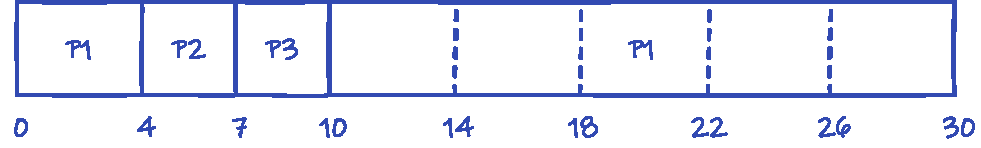
\includegraphics[width=0.8\textwidth]{media/C14_planificación/rr.pdf}
\caption{}
\end{figure}

Y los \textbf{tiempos de espera y ejecución promedio} correspondientes
serían:

\begin{longtable}[]{@{}
  >{\raggedright\arraybackslash}p{(\linewidth - 10\tabcolsep) * \real{0.2857}}
  >{\raggedright\arraybackslash}p{(\linewidth - 10\tabcolsep) * \real{0.1429}}
  >{\raggedright\arraybackslash}p{(\linewidth - 10\tabcolsep) * \real{0.1429}}
  >{\raggedright\arraybackslash}p{(\linewidth - 10\tabcolsep) * \real{0.1429}}
  >{\raggedright\arraybackslash}p{(\linewidth - 10\tabcolsep) * \real{0.1429}}
  >{\raggedright\arraybackslash}p{(\linewidth - 10\tabcolsep) * \real{0.1429}}@{}}
\toprule\noalign{}
\begin{minipage}[b]{\linewidth}\centering
Proceso
\end{minipage} & \begin{minipage}[b]{\linewidth}\centering
Instante de finalización (ms)
\end{minipage} &
\multicolumn{2}{>{\centering\arraybackslash}p{(\linewidth - 10\tabcolsep) * \real{0.2857} + 2\tabcolsep}}{\begin{minipage}[b]{\linewidth}\centering
Tiempo de espera (ms)
\end{minipage} &
\multicolumn{2}{>{\centering\arraybackslash}p{(\linewidth - 10\tabcolsep) * \real{0.2857} + 2\tabcolsep}@{}}{\begin{minipage}[b]{\linewidth}\centering
Tiempo de ejecución (ms)
\end{minipage} \\
\midrule\noalign{}
\endhead
\bottomrule\noalign{}
\endlastfoot
P1 & 30 & {(0-0) + (10-4)=} & 6 & {(30-0)=} & 24 \\
P2 & 7 & {(4-1)=} & 3 & {(7-1)=} & 6 \\
P3 & 10 & {(7-2)=} & 5 & {(10-2)=} & 8 \\
\end{longtable}

\subsubsection{Rendimiento}\label{_rendimiento}

Cuando se utiliza la planificación \textbf{RR} el tamaño del cuanto es
un factor clave en la eficiencia del planificador:

\begin{itemize}
\item
  Cuando se reduce el \textbf{cuanto}, el \textbf{tiempo de respuesta} y
  el \textbf{tiempo de espera promedio} tienden a mejorar. Sin embargo
  el número de cambios de contexto será mayor, por lo que la ejecución
  de los procesos será más lenta.

  Es importante tener en cuenta que interesa que el \textbf{cuanto} sea
  mucho mayor que el tiempo del cambio de contexto. Si, por ejemplo, el
  tiempo de cambio de contexto es un 10\% del \textbf{cuanto}, entonces
  alrededor del 10\% del tiempo de CPU se pierde en cambios de contexto.
\item
  Cuando se incrementa el \textbf{cuanto}, el \textbf{tiempo de espera
  promedio} también se incrementa. En el caso extremo en el que el
  \textbf{cuanto} es tan grande que ningún proceso lo agota, el
  \textbf{RR} se convierte en \textbf{FCFS}, que suele tener grandes
  \textbf{tiempos de espera promedio}.

  Por otro lado, puede observarse experimentalmente que el
  \textbf{tiempo de ejecución promedio} generalmente mejora cuantos más
  procesos terminan su próxima ráfaga de CPU dentro de su
  \textbf{cuanto}. Por lo tanto, nos interesa un cuanto grande para que
  más procesos terminen su siguiente ráfaga dentro del mismo.

  Dados tres procesos con una duración cada uno de ellos de 10 unidades
  de tiempo y cuanto igual a 1, el tiempo de ejecución promedio será de
  29 unidades. Sin embargo, si el cuanto de tiempo fuera 10, el tiempo
  de ejecución promedio caería a 20 unidades de tiempo.
\end{itemize}

La regla general que siguen los diseñadores es intentar que el 80\% de
las ráfagas de CPU sean menores que el tiempo de \textbf{cuanto}. Se
busca así equilibrar los criterios anteriores, evitando que el tiempo de
cuanto sea demasiado grande o demasiado corto.

Actualmente se utilizan tiempos de cuanto de entre 10 y 100 ms Estos
tiempos son mucho mayores que los tiempos de cambios de contexto, que
generalmente son inferiores a 10 µs.

\subsubsection{Reparto equitativo del tiempo de
CPU}\label{_reparto_equitativo_del_tiempo_de_cpu}

Uno de los inconvenientes del algoritmo \textbf{RR} es que no garantiza
el reparto equitativo del tiempo de CPU entre los procesos limitados por
la E/S y los limitados por la CPU ---aunque es mejor que
\textbf{FCFS}---.

Esto es debido a que los primeros utilizan el procesador durante
periodos cortos de tiempo, para bloquearse posteriormente a la espera de
que se realice la operación de E/S que han solicitado. Cuando la espera
termina, vuelven a la \textbf{cola de preparados} donde aguardan a que
se les asigne la CPU. Sin embargo, eso no va a ocurrir rápidamente si en
el sistema hay procesos limitados por la CPU, pues estos generalmente
agotan el \textbf{cuanto} antes de ser forzados a volver a la
\textbf{cola de preparados}.

Así, los procesos limitados por la CPU hacen un mayor uso de la misma,
mientras que los limitados por la E/S pueden tener que esperar durante
bastante tiempo ---aunque menos que si el algoritmo fuera \textbf{FCFS},
donde no hay \textbf{cuanto}--- en la \textbf{cola de preparados} antes
entrar en la CPU para solicitar una nueva operación de E/S. Esto hace
que se desaprovechen los dispositivos de E/S y genera un incremento de
la varianza del tiempo de respuesta. Para evitarlo se puede optar por un
\textbf{planificador de colas multinivel} ---para resolver el problema
combinando el algoritmo \textbf{RR} con otro que priorice adecuadamente
los procesos limitados por la E/S (véase el
\hyperref[_planificaciuxf3n_con_colas_multinivel]{Planificación con
colas multinivel})--- o por la \textbf{planificación equitativa} que
veremos a continuación.

\subsection{Planificación
equitativa}\label{_planificaciuxf3n_equitativa}

{} Hasta el momento hemos hablado de planificadores que se centran en
cuál es el proceso más importante para ejecutarlo a continuación. Sin
embargo, otra opción, desde el punto de vista de la planificación, es
dividir directamente el tiempo de CPU entre los procesos. Esto es
precisamente lo que hace la \textbf{planificación equitativa}
(\emph{Fair Scheduling}), que intenta repartir por igual el tiempo de
CPU entre los procesos de la cola de preparados.

Por ejemplo, supongamos que 4 procesos con diferentes ráfagas de CPU
llegan juntos y compiten por el uso de la CPU:

\begin{longtable}[]{@{}
  >{\raggedright\arraybackslash}p{(\linewidth - 2\tabcolsep) * \real{0.5000}}
  >{\raggedright\arraybackslash}p{(\linewidth - 2\tabcolsep) * \real{0.5000}}@{}}
\toprule\noalign{}
\begin{minipage}[b]{\linewidth}\centering
Proceso
\end{minipage} & \begin{minipage}[b]{\linewidth}\centering
Tiempo de ráfaga de CPU (ms)
\end{minipage} \\
\midrule\noalign{}
\endhead
\bottomrule\noalign{}
\endlastfoot
P1 & 8 \\
P2 & 4 \\
P3 & 12 \\
P4 & 4 \\
\end{longtable}

Tomando un periodo de 4 ms., en el primer periodo a cada proceso le
corresponde 1 ms. porque hay 4 procesos en estado \textbf{preparado}. Al
final del periodo 4, la ráfaga de los procesos P2 y P4 termina ---porque
ambos procesos han ejecutado 4 ms. en la CPU--- por lo que a cada uno de
los restantes le corresponden 2 ms. del periodo. Finalmente, al terminar
el periodo 6, acaba el proceso P1 ---que ya debe haberse ejecutado 8
ms.--- por lo que P4 puede usar los 4 ms. del periodo 7 y terminar
ráfaga.

En la siguiente tabla se ilustra este reparto indicando el tiempo de
cada cuanto que corresponde a cada proceso:

\begin{longtable}[]{@{}
  >{\raggedright\arraybackslash}p{(\linewidth - 14\tabcolsep) * \real{0.1250}}
  >{\raggedright\arraybackslash}p{(\linewidth - 14\tabcolsep) * \real{0.1250}}
  >{\raggedright\arraybackslash}p{(\linewidth - 14\tabcolsep) * \real{0.1250}}
  >{\raggedright\arraybackslash}p{(\linewidth - 14\tabcolsep) * \real{0.1250}}
  >{\raggedright\arraybackslash}p{(\linewidth - 14\tabcolsep) * \real{0.1250}}
  >{\raggedright\arraybackslash}p{(\linewidth - 14\tabcolsep) * \real{0.1250}}
  >{\raggedright\arraybackslash}p{(\linewidth - 14\tabcolsep) * \real{0.1250}}
  >{\raggedright\arraybackslash}p{(\linewidth - 14\tabcolsep) * \real{0.1250}}@{}}
\caption{}\label{tbl-planificaciuxf3n-equitativa-ideal}\tabularnewline
\toprule\noalign{}
\begin{minipage}[b]{\linewidth}\centering
Proceso
\end{minipage} & \begin{minipage}[b]{\linewidth}\centering
Q1
\end{minipage} & \begin{minipage}[b]{\linewidth}\centering
Q2
\end{minipage} & \begin{minipage}[b]{\linewidth}\centering
Q3
\end{minipage} & \begin{minipage}[b]{\linewidth}\centering
Q4
\end{minipage} & \begin{minipage}[b]{\linewidth}\centering
Q5
\end{minipage} & \begin{minipage}[b]{\linewidth}\centering
Q6
\end{minipage} & \begin{minipage}[b]{\linewidth}\centering
Q7
\end{minipage} \\
\midrule\noalign{}
\endfirsthead
\toprule\noalign{}
\begin{minipage}[b]{\linewidth}\centering
Proceso
\end{minipage} & \begin{minipage}[b]{\linewidth}\centering
Q1
\end{minipage} & \begin{minipage}[b]{\linewidth}\centering
Q2
\end{minipage} & \begin{minipage}[b]{\linewidth}\centering
Q3
\end{minipage} & \begin{minipage}[b]{\linewidth}\centering
Q4
\end{minipage} & \begin{minipage}[b]{\linewidth}\centering
Q5
\end{minipage} & \begin{minipage}[b]{\linewidth}\centering
Q6
\end{minipage} & \begin{minipage}[b]{\linewidth}\centering
Q7
\end{minipage} \\
\midrule\noalign{}
\endhead
\bottomrule\noalign{}
\endlastfoot
P1 & 1 & 1 & 1 & 1 & 2 & 2 & \\
P2 & 1 & 1 & 1 & 1 & & & \\
P3 & 1 & 1 & 1 & 1 & 2 & 2 & 4 \\
P4 & 1 & 1 & 1 & 1 & & & \\
\end{longtable}

Sin embargo, debemos tener en cuenta que en un instante dado, no puede
ejecutarse más de un proceso en la CPU. Es decir, durante todo el
periodo 1, realmente no pueden ejecutarse los 4 procesos al mismo
tiempo. El planificador tiene asignar la CPU en algún orden, de forma
que el tiempo finalmente usado por cada proceso en cada periodo sea
aproximadamente el calculado en la tabla anterior.

En la siguiente figura puede verse un posible reparto:

\begin{figure}
\centering
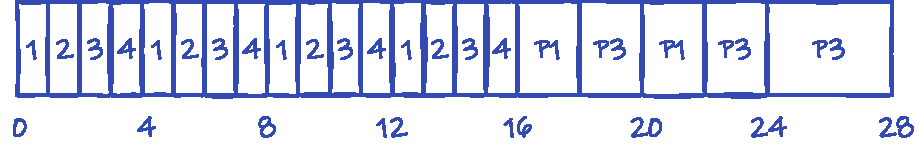
\includegraphics[width=0.8\textwidth]{media/C14_planificación/equitativo1.pdf}
\caption{}
\end{figure}

El algoritmo de \textbf{planificación equitativa} es muy similar al
algoritmo \textbf{RR}, pero en la \textbf{planificación equitativa} la
ventana de tiempo que finalmente se asigna a cada proceso se calcula
dinámicamente.

\subsubsection{Implementación
básica}\label{_implementaciuxf3n_buxe1sica}

Las implementaciones del algoritmo de \textbf{planificación equitativa}
suelen utilizar el concepto de \emph{tiempo virtual} para seguir la
pista de cuánto tiempo debe ejecutarse el proceso. Por ejemplo, en el
planificador de \{zircon\}\hyperref[Fuchsia-ZirconFairScheduler]{???}
---el \emph{microkernel} de \{google\_fuchsia\}--- cuando un proceso
\(P_i\) entra en la \textbf{cola de preparados}, en el PCB de dicho
proceso se actualizan dos tiempos:

\begin{itemize}
\item
  \textbf{Instante inicial \(t_(si)\)} de la ráfaga de CPU del proceso,
  en el \emph{tiempo virtual} de la CPU.
\item
  \textbf{Instante final \(t_(fi)\)} de la ráfaga de CPU del proceso, en
  el \emph{tiempo virtual} de la CPU.
\end{itemize}

Estos tiempos se dicen que están en \emph{tiempo virtual} de la CPU para
señalar que idealmente el proceso comenzaría su ejecución en \(t_(si)\)
y terminaría en \(t_(fi)\), aunque esto difícilmente va a ocurrir en la
realidad porque el tiempo de CPU hay que repartirlo entre los diferentes
procesos.

\{zircon\} es un \emph{microkernel} multihilo con modelo uno a uno, por
lo que su planificador trabaja con hilos. Es decir, las propiedades que
necesita el planificador para hacer su trabajo están vinculadas a los
hilos y son estos hilos los que el planificador ordena y selecciona para
ser ejecutados en la CPU. Sin embargo, en la versión que vamos a
describir hablaremos de planificar procesos, por coherencia con cómo
hemos explicado el resto de planificadores de este capítulo.

Si \(t\) es el instante de tiempo en el que un proceso \(P_i\) entra en
la cola de preparados, el instante inicial \(t_(si)\) y el instante
final \(t_(fi)\) se calculan de la siguiente manera:

\[{: (t_(si), =, t\qquad\qquad), (t_(fi), =, t_(si) + gM):}\]

donde \(M\) es la porción mínima de tiempo de CPU real que se puede
asignar a cada proceso y \(g\) es la cantidad de estas porciones de
tiempo que se quiere repartir entre todos los procesos que están en
disposición de ser ejecutados. Es decir, en el ejemplo anterior
\(gM = 4" ms"\), por lo que si la porción mínima fuera \(M = 1" ms."\),
cada periodo tendría 4 porciones de tiempo para repartir.

En la \textbf{cola de preparados} los procesos son ordenados por el
valor de \(t_(fi)\), de forma que primero se planifican los procesos que
tiene ráfagas que virtualmente terminarían antes.

El planificador de \{zircon\} tiene una serie de parámetros ajustables:

\begin{itemize}
\item
  La \textbf{granularidad mínima \(M\)} que, como hemos comentado, es la
  porción mínima de tiempo de CPU real que se puede asignar a cualquier
  proceso.
\item
  La \textbf{latencia objetivo \(L\)}, que es el periodo de tiempo de
  CPU mínimo que se va a repartir entre los procesos. Es decir, dentro
  de un periodo de \textbf{latencia objetivo} \(L\) hay
  \("floor"(L / M)\) porciones de tiempo para repartir entre los
  procesos.
\end{itemize}

Si hay \(n\) procesos que se pueden ejecutar, lo que hace el
planificador es calcular \(g\) de la siguiente manera:

\[g = max(n, "floor"(L/M))\]

de forma que siempre haya suficientes porciones \(M\) para que cada
proceso pueda tener al menos una, limitando por debajo el número de
porciones a repartir a \("floor"(L / M)\).

Cuando se escoge un proceso para su ejecución, se calcula el cuanto real
\(t_i\) durante el que se le asignará la CPU:

\[t_i = "ceil"(g/n)*M\]

de forma que se reparten las \(g\) porciones entre los \(n\) procesos.

Si hay muchos procesos, \(g = n\), por lo que a cada proceso se le
asigna un tiempo de CPU de \(M\). Si hay pocos procesos,
\(g = "floor"(L / M)\), por lo que a cada proceso se le asignan varias
porciones \(M\) de tiempo de CPU del periodo \(L\).

\subsubsection{Planificación equitativa
ponderada}\label{_planificaciuxf3n_equitativa_ponderada}

{} Al igual que en los algoritmos anteriores de planificación, en
ocasiones puede ser interesante priorizar unos procesos frente a otros,
tanto por motivos ajenos al sistema operativo como por motivos internos.
Por ejemplo, se puede querer favorecer a los procesos limitados por la
E/S para mejorar la eficiencia del sistema, tal y como comentamos en el
apartado \hyperref[_ciclo_de_ruxe1fagas_de_cpu_y_de_es]{Ciclo de ráfagas
de CPU y de E/S}.

La \textbf{planificación equitativa} resuelve este problema permitiendo
que a los procesos se les asignen pesos y repartiendo más tiempo de CPU
a los procesos con mayor peso. A esta generalización del planificador
equitativo se la conoce como \textbf{planificador equitativo ponderado}.

Linux, desde la versión 2.6.23, utiliza un tipo de \textbf{planificador
equitativo ponderado} denominado \textbf{{}CFS} (\emph{Completely Fair
Scheduler}) o \textbf{planificador completamente
equitativo}{}\hyperref[Jones2018]{???}. Otro ejemplo es \{zircon\} que,
como hemos comentado, está inmerso en cambiar su actual planificador
basado en colas multinivel con prioridades a una implementación del
\textbf{planificador equitativo} que, de hecho, es realmente un
\textbf{planificador equitativo
ponderado}\hyperref[Fuchsia-ZirconFairScheduler]{???}.

\subsubsection{Implementación de la planificación equitativa
ponderada}\label{_implementaciuxf3n_de_la_planificaciuxf3n_equitativa_ponderada}

En \{zircon\} cada proceso \(P_i\) tiene un peso \(w_i\) que indica la
importancia del proceso en el reparto del tiempo de CPU.

El primer cambio ---respecto a la implementación vista anteriormente---
es que el instante final \(t_(fi)\) realmente se calcula de la siguiente
manera:

\[t_(fi) = t_(si) + gM/w_i\]

de forma que es los procesos con mayor peso \(w_i\) tiene un \(t_(fi)\)
más pequeño, por lo que se colocan antes en la \textbf{cola de
preparados}.

Cuando se escoge un proceso para su ejecución, se calcula el cuanto real
\(t_(i)\) durante el que se le asignará la CPU, asignándole un tiempo
proporcional al peso del proceso \(w_i\) respecto al peso del resto de
los procesos con los que compite:

\[t_i = "ceil"(g*w_i/W)*M\]

donde \(W\) es la suma de todos los pesos \(w_i\) para los \(n\)
procesos preparados para ser ejecutados.

\subsubsection{Ejemplo de planificación equitativa
ponderada}\label{_ejemplo_de_planificaciuxf3n_equitativa_ponderada}

Ilustremos el algoritmo con un ejemplo con \(L=5\) y \(M=1\):

\begin{longtable}[]{@{}
  >{\raggedright\arraybackslash}p{(\linewidth - 6\tabcolsep) * \real{0.2500}}
  >{\raggedright\arraybackslash}p{(\linewidth - 6\tabcolsep) * \real{0.2500}}
  >{\raggedright\arraybackslash}p{(\linewidth - 6\tabcolsep) * \real{0.2500}}
  >{\raggedright\arraybackslash}p{(\linewidth - 6\tabcolsep) * \real{0.2500}}@{}}
\toprule\noalign{}
\begin{minipage}[b]{\linewidth}\centering
Proceso
\end{minipage} & \begin{minipage}[b]{\linewidth}\centering
Tiempo de llegada (ms)
\end{minipage} & \begin{minipage}[b]{\linewidth}\centering
Tiempo de ráfaga de CPU (ms)
\end{minipage} & \begin{minipage}[b]{\linewidth}\centering
Peso
\end{minipage} \\
\midrule\noalign{}
\endhead
\bottomrule\noalign{}
\endlastfoot
P1 & 0 & 10 & 2 \\
P2 & 1 & 2 & 1 \\
P3 & 2 & 3 & 2 \\
P4 & 3 & 2 & 5 \\
\end{longtable}

El resultado es el que se muestra en el siguiente diagrama de Gantt:

\begin{figure}
\centering
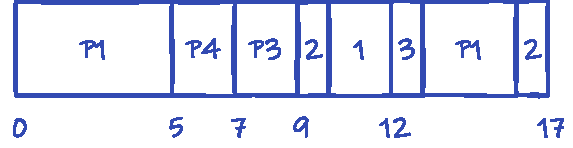
\includegraphics[width=0.8\textwidth]{media/C14_planificación/equitativo2.pdf}
\caption{}
\end{figure}

Al empezar, el primer proceso está solo cuando se le asigna la CPU, por
lo que puede consumir toda la latencia de planificación \(L\) en el
primer periodo. Posteriormente, cuando vuelve a la \textbf{cola de
preparados} en el instante 5, han llegado el resto de procesos, por lo
que tiene que competir con ellos por la CPU.

A partir de ese instante el orden para asignar la CPU viene determinado
por \(t_(fi)\), cuya expresión depende de \(g\). En este caso
\(g=M/L=5\) en todo momento, puesto que hay menos procesos que porciones
de tiempo \(M\) en \(L\).

En la siguiente tabla se puede observar los valores de \(t_(si)\) y
\(t_(fi)\) para cada proceso en el instante 5:

\begin{longtable}[]{@{}
  >{\raggedright\arraybackslash}p{(\linewidth - 4\tabcolsep) * \real{0.3333}}
  >{\raggedright\arraybackslash}p{(\linewidth - 4\tabcolsep) * \real{0.3333}}
  >{\raggedright\arraybackslash}p{(\linewidth - 4\tabcolsep) * \real{0.3333}}@{}}
\toprule\noalign{}
\begin{minipage}[b]{\linewidth}\centering
Proceso
\end{minipage} & \begin{minipage}[b]{\linewidth}\centering
\(t_(si)\)
\end{minipage} & \begin{minipage}[b]{\linewidth}\centering
\(t_(fi)\)
\end{minipage} \\
\midrule\noalign{}
\endhead
\bottomrule\noalign{}
\endlastfoot
P1 & 5 & 7.5 \\
P2 & 1 & 6 \\
P3 & 2 & 4.5 \\
P4 & 3 & 4 \\
\end{longtable}

Aunque el proceso \(P_4\) es el último en llegar, es el siguiente en ser
planificado, porque al tener un peso más alto su \(t_f4\) es el más
bajo. Entonces se calcula el tiempo de cuanto \(t_4\), que da 3, por lo
que se planifica en la CPU durante ese tiempo.

Sin embargo, \(P_4\) no consume su tiempo de cuanto porque su ráfaga
terminar antes, por lo que en el instante 7 se tiene que planificar el
siguiente proceso en la \textbf{cola de preparados}. En este caso sería
\(P_3\), con un tiempo de cuanto de 2.

Para calcular \(t_3\) es importante recordar que \(W = 5\), puesto que
\(P_4\) ya no está en la \textbf{cola de preparados} por lo que su peso
no se incluye.

En el instante 9, el proceso \(P_3\) es expulsado de la CPU y vuelve a
la \textbf{cola de preparados}. Entonces, se tienen que actualizar sus
valores para \(t_(si)\) y \(t_(fi)\) con el objeto de determinar cuál
será el próximo proceso planificado:

\begin{longtable}[]{@{}
  >{\raggedright\arraybackslash}p{(\linewidth - 4\tabcolsep) * \real{0.3333}}
  >{\raggedright\arraybackslash}p{(\linewidth - 4\tabcolsep) * \real{0.3333}}
  >{\raggedright\arraybackslash}p{(\linewidth - 4\tabcolsep) * \real{0.3333}}@{}}
\toprule\noalign{}
\begin{minipage}[b]{\linewidth}\centering
Proceso
\end{minipage} & \begin{minipage}[b]{\linewidth}\centering
\(t_(si)\)
\end{minipage} & \begin{minipage}[b]{\linewidth}\centering
\(t_(fi)\)
\end{minipage} \\
\midrule\noalign{}
\endhead
\bottomrule\noalign{}
\endlastfoot
P1 & 5 & 7.5 \\
P2 & 1 & 6 \\
P3 & 9 & 11.5 \\
\end{longtable}

Por tanto, el siguiente proceso a planificar es \(P_2\) con \(t_2 = 1\).
Y así se repite el procedimiento, sucesivamente.

Una vez resuelto el problema, los \textbf{tiempos de espera y ejecución
promedio} correspondientes serían:

\begin{longtable}[]{@{}
  >{\raggedright\arraybackslash}p{(\linewidth - 10\tabcolsep) * \real{0.2857}}
  >{\raggedright\arraybackslash}p{(\linewidth - 10\tabcolsep) * \real{0.1429}}
  >{\raggedright\arraybackslash}p{(\linewidth - 10\tabcolsep) * \real{0.1429}}
  >{\raggedright\arraybackslash}p{(\linewidth - 10\tabcolsep) * \real{0.1429}}
  >{\raggedright\arraybackslash}p{(\linewidth - 10\tabcolsep) * \real{0.1429}}
  >{\raggedright\arraybackslash}p{(\linewidth - 10\tabcolsep) * \real{0.1429}}@{}}
\toprule\noalign{}
\begin{minipage}[b]{\linewidth}\centering
Proceso
\end{minipage} & \begin{minipage}[b]{\linewidth}\centering
Instante de finalización (ms)
\end{minipage} &
\multicolumn{2}{>{\centering\arraybackslash}p{(\linewidth - 10\tabcolsep) * \real{0.2857} + 2\tabcolsep}}{\begin{minipage}[b]{\linewidth}\centering
Tiempo de espera (ms)
\end{minipage} &
\multicolumn{2}{>{\centering\arraybackslash}p{(\linewidth - 10\tabcolsep) * \real{0.2857} + 2\tabcolsep}@{}}{\begin{minipage}[b]{\linewidth}\centering
Tiempo de ejecución (ms)
\end{minipage} \\
\midrule\noalign{}
\endhead
\bottomrule\noalign{}
\endlastfoot
P1 & 16 & {(0-0) + (10-5) + (13-12)=} & 6 & {(16-0)=} & 16 \\
P2 & 17 & {(9-1) + (16-10)=} & 14 & {(17-1)=} & 16 \\
P3 & 14 & {(7-2) + (12-9)=} & 7 & {(13-2)=} & 11 \\
P4 & 7 & {(5-4)=} & 1 & {(7-3)=} & 4 \\
\end{longtable}

\subsection{Planificación con colas
multinivel}\label{_planificaciuxf3n_con_colas_multinivel}

{} Los diseñadores recurren a la \textbf{planificación de colas
multinivel} cuando quieren combinar las características de varios
algoritmos.

En la planificación con colas multinivel se divide la cola de preparados
en colas separadas. Los procesos son asignados permanentemente a alguna
de dichas colas, cada una de las cuales puede tener un algoritmo de
planificación distinto.

La asignación de un proceso a una cola se hace en relación a alguna una
característica del proceso. Por ejemplo, si es interactivo o no, su
prioridad o su tamaño en memoria. Se hace de esta manera porque se
supone que los procesos se pueden clasificar, y que cada clase tiene
diferentes requerimientos. Por ejemplo, si los procesos se clasifican en
interactivos o no interactivos, los primeros pueden ir a una cola con
planificación \textbf{RR} mientras los segundos van a una con
\textbf{FCFS}.

\begin{figure}
\centering
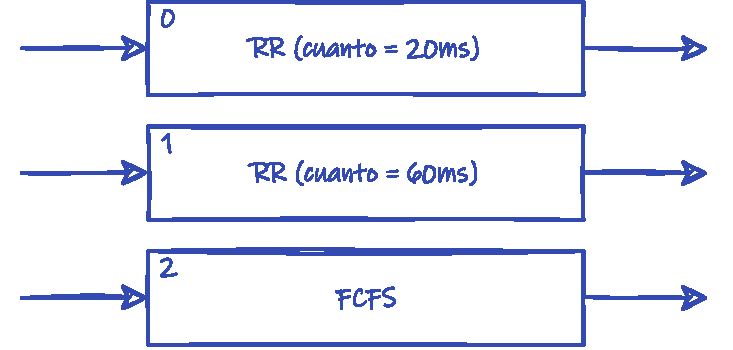
\includegraphics[width=0.8\textwidth]{media/C14_planificación/planificación_colas_multinivel.pdf}
\caption{Ejemplo de planificación con colas
multinivel.}\label{fig-colas-multinivel}
\end{figure}

Una cuestión interesante es cómo seleccionar la cola que debe escoger al
siguiente proceso a ejecutar:

\begin{itemize}
\item
  Una opción común en los sistemas actuales es utilizar un
  \textbf{planificador con prioridades}. Es decir, que cada cola tenga
  una prioridad y así el planificador solo tiene que escoger la cola de
  prioridad más alta que no esté vacía.

  Por ejemplo, en la \hyperref[fig-colas-multinivel]{Ejemplo de
  planificación con colas multinivel.}, mientras un proceso de prioridad
  1 esté preparado, no se escoge ningún otro de prioridad inferior. Si
  este planificador se implementa de forma expropiativa, el proceso que
  tiene asignada la CPU es expulsado si un proceso entra en una de las
  colas que tiene mayor prioridad que la suya.
\item
  Otra opción es usar cuantos sobre las colas. Es decir, que a cada cola
  se le asigne una porción del tiempo de la CPU que debe repartirse
  entre los distintos procesos en la misma.

  Por ejemplo, un 80\% de CPU para la cola de procesos interactivos, con
  planificación \textbf{RR}, y el 20\% de CPU restante para la cola de
  procesos no interactivos, con planificador \textbf{FCFS}.
\end{itemize}

La \textbf{planificación de colas multinivel} con un
\textbf{planificador con prioridades} para escoger la cola adecuada, es
con diferencia la opción más común en los sistemas operativos modernos.
Sin embargo, en este tipo de \textbf{colas multinivel} la asignación de
los procesos a las colas es permanente ---si la asignación se hace por
prioridad, significa que la prioridad es fija---. Mientras que hoy en
día es común que los procesos se muevan entre colas según las
características del proceso.

\subsection{Planificación con colas multinivel
realimentadas}\label{_planificaciuxf3n_con_colas_multinivel_realimentadas}

{} Para aumentar la flexibilidad de la planificación con colas
multinivel se puede permitir a los procesos pasar de una cola a otra.
Así se pueden clasificar en colas distintas, procesos con diferentes
tiempos de ráfaga de CPU. Por ejemplo, para situar los procesos
interactivos o limitados por la E/S en las colas de más alta prioridad,
lo que ya hemos discutido que mejora los tiempos de espera y de
respuesta y evita el \textbf{efecto convoy}.

\begin{figure}
\centering
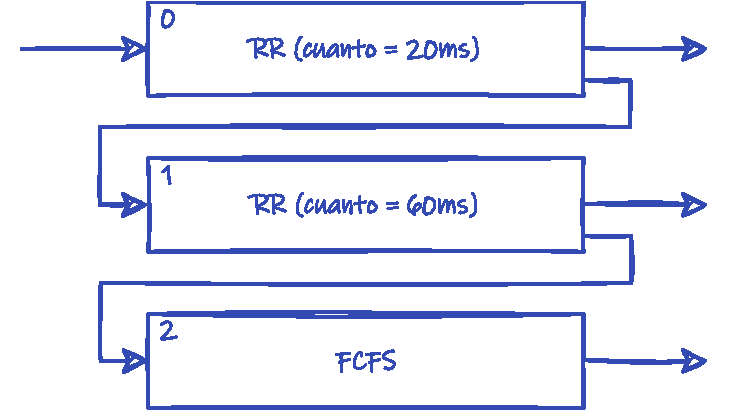
\includegraphics[width=0.8\textwidth]{media/C14_planificación/planificación_colas_multinivel_realimentadas.pdf}
\caption{Ejemplo de planificación con colas multinivel
realimentadas.}\label{fig-planificaciuxf3n-colas-multinivel-realimentadas}
\end{figure}

Por ejemplo, supongamos un \textbf{planificador de colas multinivel}
donde cada cola tiene una prioridad, así que se usa la
\textbf{planificación con prioridades} para seleccionar la cola. En las
colas se usa el algoritmo \textbf{RR} para seleccionar el siguiente
proceso, siendo el \textbf{cuanto} de la cola mayor cuanto menos
prioritaria es la cola (véase la
\hyperref[fig-planificaciuxf3n-colas-multinivel-realimentadas]{Ejemplo
de planificación con colas multinivel realimentadas.}). Los procesos que
llegan nuevos o desde el estado \textbf{esperando} lo hacen con la
prioridad más alta ---que por convención hemos decidido que sea 0--- así
que se insertan en la cola correspondiente. Mientras que los procesos
expropiados por vencimiento del \textbf{cuanto} pierde un punto de
prioridad, siendo insertados en una cola de prioridad menor.

Con este algoritmo los procesos limitados por E/S suelen ejecutarse la
mayor parte del tiempo con prioridades más altas que los limitados por
CPU. Por ejemplo, usando los valores del esquema de la
\hyperref[fig-planificaciuxf3n-colas-multinivel-realimentadas]{Ejemplo
de planificación con colas multinivel realimentadas.}, los procesos de
ráfagas de CPU entre 20 y 80 ms acaban cayendo a la cola de prioridad 1
tras 20 ms de ejecución. Así dejan paso a los procesos con ráfagas
menores de 20 ms, que siempre se ejecutan con prioridad 0. Finalmente,
los procesos de ráfagas mayores de 80 ms van a la cola FCFS, desde donde
solo tendrán acceso a la CPU cuando no haya ningún proceso de los otros
tipos en la \textbf{cola de preparados}

El \textbf{planificador de colas multinivel realimentadas} también se
puede utilizar para pasar a colas superiores los procesos que han
esperado mucho tiempo en colas inferiores, evitando la \textbf{muerte
por inanición}, que puede afectar a los sistemas de
\textbf{planificación de colas multinivel} con \textbf{prioridad fija}.

Por ejemplo, el algoritmo \textbf{RR virtual}{}{} es un caso de
\textbf{planificador de colas multinivel realimentadas} que resuelve los
problemas del \textbf{RR}, en cuanto al reparto de la CPU entre procesos
limitados por la E/S y limitados por la CPU (véase el
\hyperref[_reparto_equitativo_del_tiempo_de_cpu]{Reparto equitativo del
tiempo de CPU}).

\begin{figure}
\centering
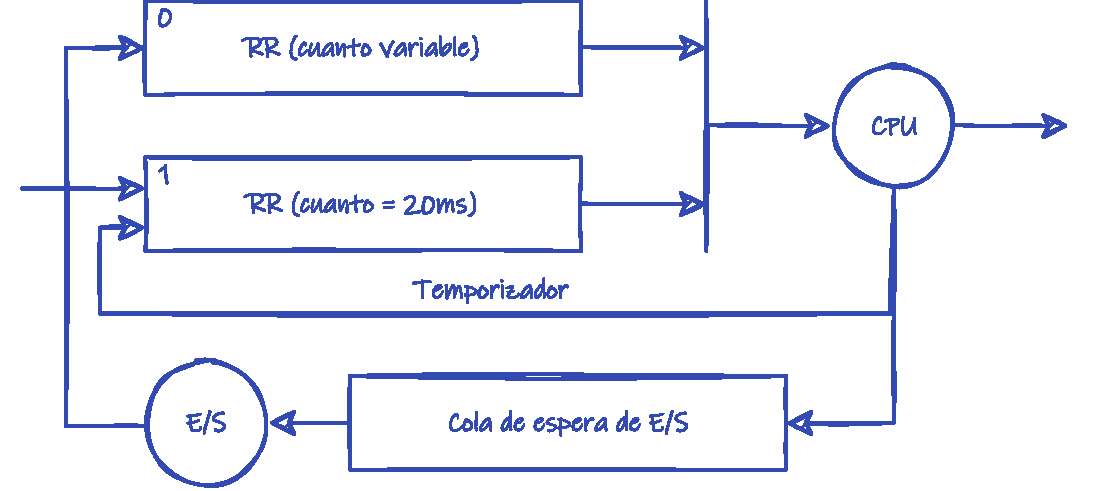
\includegraphics[width=0.8\textwidth]{media/C14_planificación/vrr.pdf}
\caption{Ejemplo de planificación con RR
virtual.}\label{fig-planificaciuxf3n-rr-virtual}
\end{figure}

Tal y como se ilustra en la
\hyperref[fig-planificaciuxf3n-rr-virtual]{Ejemplo de planificación con
RR virtual.}, en el \textbf{RR virtual} los procesos por lo general
tienen prioridad 1. Sin embargo, aquellos que vuelven al estado
\textbf{preparado} desde \textbf{esperando} después de una operación de
E/S, obtienen una bonificación en la propiedad que los lleva a tener
prioridad 0. Por tanto, los procesos que usan con más frecuencia la E/S,
usan más la cola de prioridad más alta, por lo que se les asigna antes
la CPU mayor frecuencia.

Esta solución puede llevar a que si hay muchos procesos limitados por la
E/S, estos acaparen la CPU y no den oportunidad de ejecutarse a los
procesos en la cola de prioridad 1. Para evitarlo, el algoritmo
\textbf{RR} de la cola de prioridad 0 tiene un \textbf{cuanto} variable,
de tal forma que cada proceso recibe lo que le queda del \textbf{cuanto}
de la cola de prioridad 1 tras haber consumido parte en la CPU en la
ráfaga anterior. Esto hace que incluso los procesos con ráfagas de CPU
más cortas acaben consumiendo su \textbf{cuanto} en la cola de prioridad
0 y terminen cayendo a la cola de prioridad 1, dando oportunidad de
ejecutarse a otros procesos.

Para ilustrar los visto hasta el momento sobre la planificación de la
CPU en sistemas operativos modernos, vamos a comentar las principales
características de las últimas versiones de Microsoft Windows a este
respecto.

Las actuales versiones de sistemas operativos Windows pertenecen a la
familia de Microsoft Windows NT; que nació con el sistema operativo
Windows NT 3.1 en 1993 y que llega hasta hoy en día con Microsoft
Windows 10 y Windows Server 2019 ---que se corresponden con la versión
10.0 de dicha familia Windows NT---

El núcleo de la familia Windows NT es multihilo e internamente
implementa un algoritmo de planificación expropiativa con colas
multinivel realimentadas basado en prioridades.

En Windows las prioridades de los hilos se pueden ver desde dos
perspectivas: la de Windows API y la del núcleo. Ambas tienen una
organización muy diferente, pero en última instancia, las primeras deben
traducirse en las segundas.

\begin{longtable}[]{@{}
  >{\raggedright\arraybackslash}p{(\linewidth - 2\tabcolsep) * \real{0.5000}}
  >{\raggedright\arraybackslash}p{(\linewidth - 2\tabcolsep) * \real{0.5000}}@{}}
\caption{Clases de prioridad en Windows
API.}\label{tabla-win32-clases-prioridad}\tabularnewline
\toprule\noalign{}
\begin{minipage}[b]{\linewidth}\centering
Clase
\end{minipage} & \begin{minipage}[b]{\linewidth}\centering
Valor
\end{minipage} \\
\midrule\noalign{}
\endfirsthead
\toprule\noalign{}
\begin{minipage}[b]{\linewidth}\centering
Clase
\end{minipage} & \begin{minipage}[b]{\linewidth}\centering
Valor
\end{minipage} \\
\midrule\noalign{}
\endhead
\bottomrule\noalign{}
\endlastfoot
REALTIME\_PRIORITY\_CLASS & 0x00000100 \\
HIGH\_PRIORITY\_CLASS & 0x00000080 \\
ABOVE\_NORMAL\_PRIORITY\_CLASS & 0x00008000 \\
NORMAL\_PRIORITY\_CLASS & 0x00000020 \\
BELOW\_NORMAL\_PRIORITY\_CLASS & 0x00004000 \\
IDLE\_PRIORITY\_CLASS & 0x00000040 \\
\end{longtable}

Desde el punto de vista de Windows API, todo proceso pertenece a alguna
de las 6 clases de prioridad de la
\hyperref[tabla-win32-clases-prioridad]{Clases de prioridad en Windows
API.}\hyperref[Win32-SchedulingPriorities]{???}. La clase de prioridad
de un proceso se puede indicar durante la creación del proceso, a través
del argumento \texttt{dwCreationFlags} de la función
\{win32\_createprocess\}, o sea puede obtener y cambiar con las
funciones \{win32\_getpriorityclass\} y \{win32\_setpriorityclass\},
respectivamente. Por lo general, la clase de prioridad
\texttt{NORMAL\_PRIORITY\_CLASS} es la clase por defecto de cualquier
proceso nuevo, excepto que se indique otra cosa durante su creación.

\begin{figure}
\centering
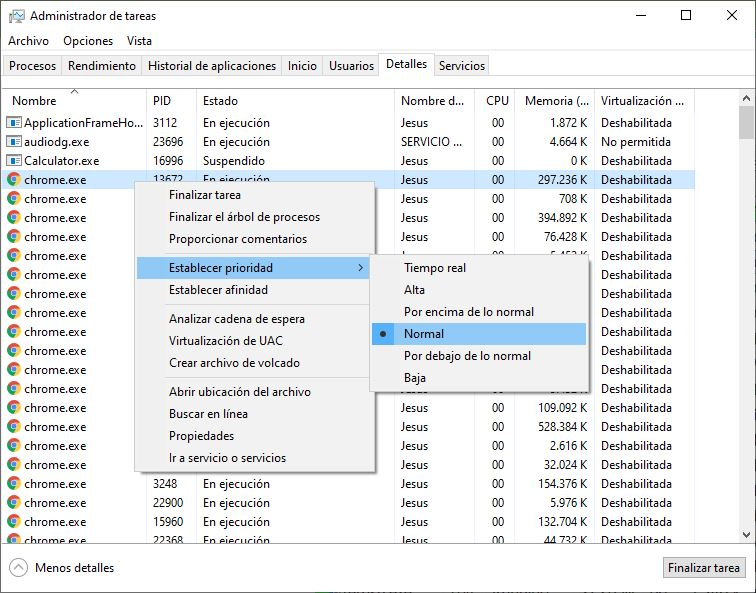
\includegraphics[keepaspectratio]{media/C14_planificación/administrador_de_tareas.jpg}
\caption{Cambiar la prioridad de un proceso en el \textbf{Administrador
de tareas}.}\label{fig-windows-task-manager}
\end{figure}

Con el \textbf{Administrador de tareas} de Windows podemos alterar
fácilmente la clase de prioridad de un proceso durante su ejecución
(véase la \hyperref[fig-windows-task-manager]{Cambiar la prioridad de un
proceso en el .}).

\begin{longtable}[]{@{}
  >{\raggedright\arraybackslash}p{(\linewidth - 2\tabcolsep) * \real{0.5000}}
  >{\raggedright\arraybackslash}p{(\linewidth - 2\tabcolsep) * \real{0.5000}}@{}}
\caption{Clases de prioridad en Windows
API.}\label{tabla-win32-prioridad-hilos}\tabularnewline
\toprule\noalign{}
\begin{minipage}[b]{\linewidth}\centering
Prioridad
\end{minipage} & \begin{minipage}[b]{\linewidth}\centering
Valor
\end{minipage} \\
\midrule\noalign{}
\endfirsthead
\toprule\noalign{}
\begin{minipage}[b]{\linewidth}\centering
Prioridad
\end{minipage} & \begin{minipage}[b]{\linewidth}\centering
Valor
\end{minipage} \\
\midrule\noalign{}
\endhead
\bottomrule\noalign{}
\endlastfoot
THREAD\_PRIORITY\_TIME\_CRITICAL & 15 \\
THREAD\_PRIORITY\_HIGHEST & 2 \\
THREAD\_PRIORITY\_ABOVE\_NORMAL & 1 \\
THREAD\_PRIORITY\_NORMAL & 0 \\
THREAD\_PRIORITY\_BELOW\_NORMAL & -1 \\
THREAD\_PRIORITY\_LOWEST & -2 \\
THREAD\_PRIORITY\_IDLE & 15 \\
\end{longtable}

Al mismo tiempo, cada hilo del sistema tiene alguno de las prioridades
de la \hyperref[tabla-win32-prioridad-hilos]{Clases de prioridad en
Windows API.}. La prioridad de un hilo recién creado es
\texttt{THREAD\_PRIORITY\_NORMAL}, pero se puede cambiar usando la
función \{win32\_setthreadpriority\}.

El núcleo de Windows tiene 32 prioridades, siendo 31 la prioridad más
alta y 0 la más baja. Estos valores se dividen en dos rangos. El rango
de prioridades de tiempo real va de 16 a 31 y solo está disponible para
hilos en procesos en la clase de prioridad
\texttt{REALTIME\_PRIORITY\_CLASS}. Mientras que el rango de prioridades
dinámicas va de 1 a 15. El nivel 0 está reservado para el sistema y se
usa para una rutina especializada en limpiar zonas de memoria liberada
por los procesos, poniéndolas a 0.

La prioridad base ---o prioridad estática--- de cada hilo que ve el
núcleo se calcula combinando la prioridad del hilo y la clase de
prioridad del proceso al que pertenece.

\begin{longtable}[]{@{}
  >{\raggedright\arraybackslash}p{(\linewidth - 12\tabcolsep) * \real{0.1429}}
  >{\raggedright\arraybackslash}p{(\linewidth - 12\tabcolsep) * \real{0.1429}}
  >{\raggedright\arraybackslash}p{(\linewidth - 12\tabcolsep) * \real{0.1429}}
  >{\raggedright\arraybackslash}p{(\linewidth - 12\tabcolsep) * \real{0.1429}}
  >{\raggedright\arraybackslash}p{(\linewidth - 12\tabcolsep) * \real{0.1429}}
  >{\raggedright\arraybackslash}p{(\linewidth - 12\tabcolsep) * \real{0.1429}}
  >{\raggedright\arraybackslash}p{(\linewidth - 12\tabcolsep) * \real{0.1429}}@{}}
\caption{Clases de prioridad base en Windows
API.}\label{tabla-win32-prioridad-estuxe1tica}\tabularnewline
\toprule\noalign{}
\endfirsthead
\endhead
\bottomrule\noalign{}
\endlastfoot
&
\multicolumn{6}{>{\centering\arraybackslash}p{(\linewidth - 12\tabcolsep) * \real{0.8571} + 10\tabcolsep}@{}}{\textbf{Clase de prioridad del proceso}} \\
& \textbf{REALTIME} & \textbf{HIGH} & \textbf{ABOVE NORMAL} &
\textbf{NORMAL} & \textbf{BELOW NORMAL} & \textbf{IDLE} \\
\textbf{TIME CRITICAL} & 31 & 15 & 15 & 15 & 15 & 15 \\
\textbf{HIGHEST} & 26 & 15 & 12 & 10 & 8 & 6 \\
\textbf{ABOVE NORMAL} & 25 & 15 & 11 & 9 & 7 & 6 \\
\textbf{NORMAL} & 24 & 13 & 10 & 8 & 6 & 4 \\
\textbf{BELOW NORMAL} & 23 & 12 & 9 & 7 & 5 & 3 \\
\textbf{LOWEST} & 22 & 11 & 8 & 6 & 4 & 2 \\
\textbf{IDLE} & 16 & 1 & 1 & 1 & 1 & 1 \\
\end{longtable}

Esta prioridad base es la prioridad real del hilo, si este tiene una
prioridad en el rango de tiempo real ---es decir, si el proceso al que
pertenece está en la clase de prioridad
\texttt{REALTIME\_PRIORITY\_CLASS}---. Mientras que para el resto de
hilos, el sistema suma ciertas bonificaciones a la prioridad base para
calcular la prioridad dinámica, que es con la que realmente será
planificado el hilo. Estas bonificaciones se truncan para que nunca
puedan hacer que el hilo se meta en el rango de tiempo real.

La prioridad real la usa el sistema para determinar a qué cola va el
hilo cuando va a ser insertado en la \textbf{cola de preparados}. Para
cada nivel de prioridad hay una cola con algoritmo \textbf{RR}, de tal
forma que el planificador escoge primero a los hilos con prioridad más
alta. Dentro de la misma prioridad la CPU se asigna en turno, dándoles
un \textbf{cuanto} de tiempo de CPU.

Cuando llega un hilo a la cola de preparados, expropia la CPU al hilo
que la tiene asignada si este tiene menor prioridad. Esto puede ocurrir
incluso si el hilo a expropiar está en medio de una llamada al sistema,
ya que, como cualquier sistema operativo moderno, el núcleo de Windows
es expropiable ---lo que veremos en el
\hyperref[_nuxfacleo_expropiable]{Núcleo expropiable} que ofrece
latencias de asignación más bajas que si no lo fuera---.

Respecto al \textbf{cuanto}, desde Windows Vista --NT 6.0-- no se usa el
temporizador para controlarlo sino el contador de ciclos de reloj de la
CPU. Así el sistema puede determinar con precisión el tiempo que se ha
estado ejecutando un hilo, excluyendo los tiempos dedicados a otras
cuestiones, como por ejemplo a manejar interrupciones.

Desde el Intel Pentium las CPU de la familia x86 incorporan un contador
de marca de tiempo (\emph{Time Stamp Counter} o TSC) de 64 bits que
indica el número de ciclos transcurridos desde el último reinicio del
procesador\hyperref[Wikipedia-TSC]{???}.

Una característica curiosa es que los hilos expropiados se insertan en
la cabeza de su cola ---no en el final--- y conservan lo que les queda
de \textbf{cuanto}. Mientras que se insertan por el final con el valor
de \textbf{cuanto} reiniciado cuando abandonan la CPU por haber agotado
el cuanto anterior. Estos últimos, además, pierden un nivel de prioridad
si se ejecutaban con una prioridad superior a su prioridad base, a causa
de alguna modificación.

Las bonificaciones a los hilos en el rango de prioridades dinámicas
vienen determinadas por distintos criterios, escogidos para mejorar el
\textbf{tiempo respuesta} y el \textbf{tiempo de espera} ---priorizando
los procesos limitados por E/S--- evitar la \textbf{muerte por
inanición} y la \textbf{inversión de prioridad}.

Se bonifican los hilos que despiertan tras completar operaciones de E/S
con una cantidad que depende del tipo de dispositivo. Por ejemplo, la
bonificación es mejor para hilos que han esperado por el teclado o el
ratón que para los que esperaron por dispositivos del almacenamiento.
También son bonificados los hilos que despiertan de eventos, semáforos y
de otros objetos de sincronización. En este último caso, incluso se les
ofrece más tiempo de \textbf{cuanto} si es el hilo asociado a la ventana
de primer plano, con el objetivo de mejorar la respuesta de las
aplicaciones interactivas. También se bonifica cualquier hilo que
gestione elementos de la interfaz gráfica cuando despierta para
responder a eventos del sistema de ventanas.

Para evitar la \textbf{muerte por inanición}, el planificador escoge
cada segundo unos pocos hilos que llevan esperando aproximadamente 4
segundos, les triplica el \textbf{cuanto} y les aumenta la prioridad a
15. Estos hilos recuperan su prioridad base y el cuanto anterior cuando
agotan el tiempo de cuanto actual o son expropiados de la CPU

\section{Planificación de tiempo
real}\label{_planificaciuxf3n_de_tiempo_real}

En el \hyperref[_sistemas_de_tiempo_real]{???} discutimos la importancia
de los sistemas de tiempo real. A continuación, describiremos las
funcionalidades necesarias para soportar la ejecución de procesos en
tiempo real dentro de un sistema operativo de propósito general.

\subsection{Tiempo real estricto}\label{_tiempo_real_estricto}

{} {} {} Los sistemas de \textbf{tiempo real estricto} son necesarios
para realizar tareas críticas que deben ser completadas dentro de unos
márgenes de tiempo preestablecidos.

Generalmente las tareas son entregadas al sistema operativo junto con
una declaración de las restricciones de tiempo ---periodicidad y límite
de tiempo--- y la cantidad de tiempo que necesitan para ejecutarse. El
planificador solo admitirá las tareas si puede garantizar el
cumplimiento de las restricciones de tiempo, rechazándolas en caso
contrario.

El ofrecer estas garantías requiere que el planificador conozca
exactamente el tiempo máximo que se tarda en realizar todas y cada una
de las funciones del sistema operativo. Esto es imposible en sistemas
con almacenamiento secundario o memoria virtual, ya que introducen
variaciones no controladas en la cantidad de tiempo necesario para
ejecutar una tarea. Por tanto, el \textbf{tiempo real estricto} no es
compatible con los sistemas operativos de propósito general, como los
sistemas operativos de escritorio modernos.

\subsection{Tiempo real flexible}\label{_tiempo_real_flexible}

{} {} {} La ejecución de procesos de \textbf{tiempo real flexible} es
menos restrictiva. Tan solo requiere que los procesos críticos reciban
mayor prioridad que los que no lo son. Esto puede generar excesos en la
cantidad de recursos asignados a los procesos de tiempo real, así como
inanición y grandes retrasos en la ejecución del resto de los procesos,
pero es compatible con los sistemas de propósito general.

Además nos permite conseguir sistemas de propósito general que soporten
multimedia, videojuegos y otras tareas que no funcionan de manera
aceptable en un entorno que no implementara tiempo real flexible. Por
ello, la mayor parte de los sistemas operativos modernos soportan este
tipo de tiempo real.

\subsection{Implementación del soporte de tiempo
real}\label{_implementaciuxf3n_del_soporte_de_tiempo_real}

Implementar el soporte de tiempo real flexible en un sistema operativo
de propósito general requiere:

\begin{itemize}
\item
  \textbf{Sistema operativo con planificación con prioridades}. Los
  procesos de tiempo real deben tener la mayor prioridad y ser fija. Es
  decir, no deben ser afectados por ningún mecanismo de envejecimiento o
  bonificación, que pueda usarse con los procesos de tiempo no real.
\item
  \textbf{Baja latencia de asignación}. Cuanto menor es la latencia, más
  rápido comenzará a ejecutarse el proceso de tiempo real después de ser
  seleccionado por el planificador de la CPU.
\end{itemize}

Mientras que el primer requerimiento es bastante sencillo de conseguir,
el segundo es mucho más complejo.

\subsection{Reducir la latencia de
asignación}\label{_reducir_la_latencia_de_asignaciuxf3n}

Muchos sistemas operativos tienen un núcleo no expropiable. Estos
núcleos no pueden realizar un cambio de contexto mientras se está
ejecutando código del núcleo ---por ejemplo, debido a una llamada al
sistema--- por lo que se ven obligados a esperar hasta que la operación
que se esté realizando termine, antes de asignar la CPU a otro proceso.
Esto aumenta la \textbf{latencia de asignación}, dado que algunas
llamadas al sistema pueden ser muy complejas y requerir mucho tiempo
para completarse.

Con el objetivo de resolver este problema se han desarrollado diversas
alternativas para que el código del núcleo sea expropiable.

\subsubsection{Puntos de expropiación}\label{_puntos_de_expropiaciuxf3n}

Una posibilidad es introduciendo \textbf{puntos de expropiación}{} en
diversos lugares «seguros» dentro del código. En dichos puntos se
comprueba si algún proceso de prioridad más alta está en la cola de
preparados. En caso de que sea así, se expropia la CPU al proceso actual
y se le asigna al proceso de más alta prioridad.

Debido a la función que realizan los puntos de expropiación, solo pueden
ser colocados en lugares seguros del código del núcleo. Es decir,
lugares donde no se interrumpe la modificación de estructuras de datos.
Sin embargo, esto limita el número de puntos que pueden ser colocados,
por lo que la latencia de asignación puede seguir siendo muy alta para
algunas operaciones muy complejas del núcleo.

\subsubsection{Núcleo expropiable}\label{_nuxfacleo_expropiable}

Otra posibilidad es diseñar un \textbf{núcleo completamente
expropiable}.

Puesto que en este caso la ejecución de cualquier operación en el núcleo
puede ser interrumpida en cualquier momento por procesos de mayor
prioridad que el que actualmente tiene asignada la CPU, es necesario
proteger las estructuras de datos del núcleo con mecanismos de
sincronización. Esto hace que el diseño de un núcleo de estas
características sea mucho más complejo.

Microsoft Windows ---desde Windows NT--- Linux ---desde la versión
2.6--- \{solaris\} y \{netbsd\} son algunos ejemplos de sistemas
operativos con núcleos expropiables. En el caso concreto de Solaris la
latencia de asignación es inferior a 1 ms, mientras que con la
expropiación del núcleo desactivada esta puede superar los 100 ms

Lamentablemente, conseguir baja latencia de asignación no tiene coste
cero. El hecho de que el núcleo sea expropiable aumenta el número de
cambios de contexto, lo que reduce el rendimiento del sistema a cambio
de un menor tiempo de respuesta. Esto resulta muy interesante para
aplicaciones de tiempo real, multimedia y sistemas de escritorio, pero
es poco adecuado para servidores y computación de altas prestaciones.

Por eso desde Linux 2.6 se puede compilar el núcleo con diferentes
niveles, de lo expropiable que es el núcleo.

En la configuración por defecto \texttt{PREEMPT\_NONE}, el núcleo tiene
algunos \textbf{puntos de expropiación}, de tal forma que es ideal para
servidores y sistemas cómputo de altas prestaciones. Con
\texttt{PREEMPT\_VOLUNTARY} ---el siguiente nivel--- se añaden muchos
más \textbf{puntos de expropiación} con el objeto de reducir la
latencia, mejorando el tiempo de respuesta en sistemas de escritorio.

Finalmente, activando \texttt{PREEMPT} el núcleo se vuelve
\textbf{completamente expropiable} ---excepto en algunas secciones
críticas---. Esto es ideal para sistemas de escritorio o sistemas
empotrados con requisitos de latencia en el rango de los milisegundos.

\paragraph{Inversión de prioridad}\label{_inversiuxf3n_de_prioridad}

Supongamos que en un núcleo completamente expropiable, un proceso de
baja prioridad es interrumpido porque hay un proceso de alta prioridad
en la cola de preparados. Y que esto ocurre mientras el primero accede a
una importante estructura de datos del núcleo.

Durante su ejecución, el proceso de alta prioridad podría intentar
acceder a la misma estructura que trataba de manipular el proceso de
baja prioridad cuando fue interrumpido. Debido al uso de mecanismos de
sincronización, el proceso de alta prioridad se quedaría bloqueado y
tendría que abandonar la CPU a la espera de que el de baja, libere el
acceso al recurso. Sin embargo, este último tardará en ser asignado a la
CPU mientras haya algún otro proceso de alta prioridad en la cola de
preparados.

Al hecho de que un proceso de alta prioridad tenga que esperar por uno
de baja se le conoce como \textbf{{}inversión de la prioridad}. Para
resolverlo se utiliza un \textbf{{}protocolo de herencia de la
prioridad}, donde un proceso de baja prioridad hereda la prioridad del
proceso de más alta prioridad que espera por un recurso al que el
primero está accediendo. En el momento en que el proceso de baja
prioridad libere el acceso a dicho recurso, su prioridad retornará a su
valor original.

\section{Planificación en sistemas
multiprocesador}\label{_planificaciuxf3n_en_sistemas_multiprocesador}

Para tratar el problema de la planificación en los sistemas
multiprocesador nos limitaremos al caso de los \textbf{sistemas
homogéneos}{}. En dichos sistemas los procesadores son idénticos, por lo
que, en cualquiera de ellos, puede ejecutar cualquier proceso. Esto es
bastante común y simplifica el problema de la planificación.

Un ejemplo de lo contrario a un sistema homogéneo ---un sistema
heterogéneo--- se puede observar en los PC modernos, donde muchos
disponen tanto de una CPU como de una GPU, especializada en el
procesamiento de gráficos y en las operaciones vectoriales con números
enteros y de coma flotante.

Aun así, no debemos olvidar que incluso en el caso de los sistemas
homogéneos pueden aparecer limitaciones en la planificación. Por
ejemplo, los procesadores SMT (\emph{Simultaneous Multithreading})
permiten la ejecución concurrente de varios hilos de ejecución como si
de varias CPU se tratara. Sin embargo, al no disponer cada hilo de una
CPU completa, es posible que algunos debán esperar a que algún otro
libere unidades de ejecución de la CPU que le son necesarias. Eso debe
ser tenido en cuenta por el planificador con el fin de optimizar el
rendimiento del sistema.

La tecnología \emph{Hyper-threading} disponible en algunos procesadores
de Intel es una implementación de la tecnología \emph{Simultaneous
Multithreading}. Permite que cada núcleo de procesador que está presente
físicamente, el sistema operativo lo gestione como dos núcleos virtuales
---o lógicos--- y repartir entre ellos las tareas cuando es posible.

Al margen de estas cuestiones, según el tipo de procesamiento, existen
diversas posibilidades a la hora de enfrentar el problema de la
planificación en un sistema multiprocesador (véase el
\hyperref[_sistemas_multiprocesador]{???}).

\subsection{Multiprocesamiento
asimétrico}\label{_multiprocesamiento_asimuxe9trico}

{} {} Cuando utilizamos \textbf{multiprocesamiento asimétrico} todas las
decisiones de planificación, procesamiento de E/S y otras actividades
son gestionadas por el núcleo del sistema ejecutándose en un único
procesador: el \textbf{servidor} o \textbf{maestro}. El resto de
procesadores se limitan a ejecutar código de usuario, que les es
asignado por ese procesador \textbf{maestro}.

Este esquema es sencillo, puesto que evita la necesidad de compartir
estructuras de datos entre el código que se ejecuta en los diferentes
procesadores.

\subsection{Multiprocesamiento
simétrico}\label{_multiprocesamiento_simuxe9trico}

{} {} Cuando utilizamos \textbf{multiprocesamiento simétrico} o
\textbf{SMP}, cada procesador ejecuta su propia copia del núcleo del
sistema operativo y se autoplanifica mediante su propio planificador de
CPU. En estos sistemas nos podemos encontrar con varias alternativas.

\subsubsection{Con una cola de preparados
común}\label{_con_una_cola_de_preparados_comuxfan}

Algunos sistemas disponen de una cola de preparados común para todos los
procesadores. Puesto que se mira en una única cola, todos los procesos
pueden ser planificados en cualquier procesador.

Este esquema requiere el uso mecanismos de sincronización para controlar
el acceso concurrente de los núcleos a las colas. En caso contrario,
varios procesadores podrían escoger y ejecutar el mismo proceso a la
vez.

Muchos sistemas operativos modernos implementan el esquema SMP con una
cola de preparados común. Esto incluye Microsoft Windows NT/2000/XP,
Solaris, macOS y versiones anteriores a Linux 2.6.

Es importante recordar que en esos sistemas operativos, lo que se
planifica en las distintas CPU usando alguna de estas estrategias, son
los hilos y no los procesos.

Sin embargo, esta solución presenta algunos inconvenientes:

\begin{itemize}
\item
  La posibilidad de que un proceso se pueda ejecutar en cualquier CPU
  ---aunque parezca beneficiosa--- es negativa desde el punto de vista
  de que dejan de ser útiles las cachés de los procesadores, penalizando
  notablemente el rendimiento del sistema. Por eso, la mayoría de los
  sistemas operativos de este tipo evitan, en lo posible, la migración
  de procesos de un procesador a otro. A esto se lo conoce como asignar
  al proceso \textbf{{}afinidad al procesador}.
\item
  Los mecanismos de sincronización requeridos para controlar el acceso a
  la cola de preparados pueden mantener a los procesadores mucho tiempo
  desocupados ---mientras esperan--- en sistemas con un gran número de
  procesadores y con muchos procesos en la cola de preparados.
\end{itemize}

\subsubsection{Con una cola para cada
procesador}\label{_con_una_cola_para_cada_procesador}

Cada vez más sistemas modernos están optando por utilizar el esquema SMP
con una cola de preparados por procesador. De esta manera, al no
utilizar mecanismos de sincronización, se eliminan los tiempos de espera
para acceder a la cola de preparados y escoger un nuevo proceso.

El mayor inconveniente de esta solución es que puede generar
desequilibrios entre los procesadores, ya que un procesador puede acabar
desocupado ---con su cola de preparados vacía--- mientras otro está muy
ocupado. Con el fin de que esto no suceda, es necesario que el sistema
disponga de algunos mecanismos de \textbf{balanceo de carga}:

\begin{itemize}
\item
  En la \textbf{migración comandada}{} o \emph{push migration}, una
  tarea específica ---que se ejecuta con menor frecuencia que el
  planificador de la CPU--- estima la carga de trabajo de cada CPU y en
  caso de encontrar algún desequilibrio mueve algunos procesos de la
  cola de preparados de unos procesadores a la de los otros.
\item
  En la \textbf{migración solicitada}{} o \emph{pull migration}, un
  procesador inactivo extrae de la cola de preparados de un procesador
  ocupado alguna tarea que esté esperando.
\end{itemize}

Tanto el planificador de Linux 2.6 y posteriores, como el planificador
ULE de FreeBSD, implementan ambas técnicas. Mientras que en Microsoft
Windows, a partir de Windows Vista también se utiliza una cola de
preparados por procesador, pero solo implementa la \textbf{migración
solicitada}.
